\chapter{Occurrence Graph Grammars}\label{ch:process}

Occurrence graph grammars were defined for the Single-Pushout (SPO) approach by~\cite{Ribeiro1996}, and for the Double-Pushout (DPO) approach by~\cite{Corradini1996}. In both cases they consist of a way of representing the concurrent semantics of a graph grammar as a graph grammar. 

The aim of an occurrence graph grammar is to describe all possible states and changes of states of the graph grammar from which the occurrence graph grammar was constructed. This is possible because occurrence grammars can be viewed as the entire execution history of the underlying grammar. This history is encoded under the forms of (1) a \emph{core graph} containing all elements ever used in the execution of a grammar and (2) a set of \emph{relations} between the rules and elements of this core graph. 

The relations can be used to express dependencies among the core graph elements, such as which of them must occur together, i.e. at the same state, which ones must be created/deleted one after the other, which elements must never occur together, and so on. They also encode restrictions over the application of rules, e.g. which rules are sequentially dependent on others, whether it is possible to successfully apply all the rules of a grammar. This property makes occurrence graph grammars excellent
candidates for the generation of test cases, as we are interested in a way of representing several (equivalent) possible derivations using a compact notation.

However, Negative Application Conditions are not addressed by the original definitions of occurrence grammars. Still, NACs are nowadays essential for modelling complex systems as graph grammars, since they provide more possibilities to control the application of rules~\cite{Habel1996, Lambers2008, Corradini2014}.

In order to use this framework for our purposes, we first need to extend occurrence grammars in order to contemplate negative application conditions. Thus, in the next sections we review the works done by~\cite{Ribeiro1996} and~\cite{Corradini1996} in occurrence graph grammars, after which we propose an extension to deal with NACs.

\section{Occurrence Graph Grammars}

\begin{definition}[Doubly-Typed Graph] Given a type graph $T$, a \emph{doubly-typed graph} \doublyTypedGraph{} over $T$ is a tuple \doublyTypedGraph $= \left(G^T,TG^T, t^{G^T} : G^T \rightarrow TG^T\right)$ where $G^T$ and $TG^T$ are typed graphs over $T$ and \mbox{$t^{G^T} : G^T \rightarrow TG^T$} is a typed graph morphism in \typedGraphCategory{}. We call $TG^T$ the \emph{double-type graph} and $t^{G^T}$ the double-typing morphism.
\end{definition}

\begin{remark}[Typing Morphism] In this work, we will consider only doubly-typed graphs whose typing morphism $type_{TG} : TG \rightarrow T$ is an epimorphism. This has the effect that every element present in $T$ is the image of at least one element from $TG$.
\end{remark}

\begin{example}[Doubly-Typed Graph Example] Figure~\ref{fig:process:doubly-typed-graph} shows a doubly-typed graph $G^{TG^T}$.

\begin{figure}[!ht]
  \centering
  \fbox{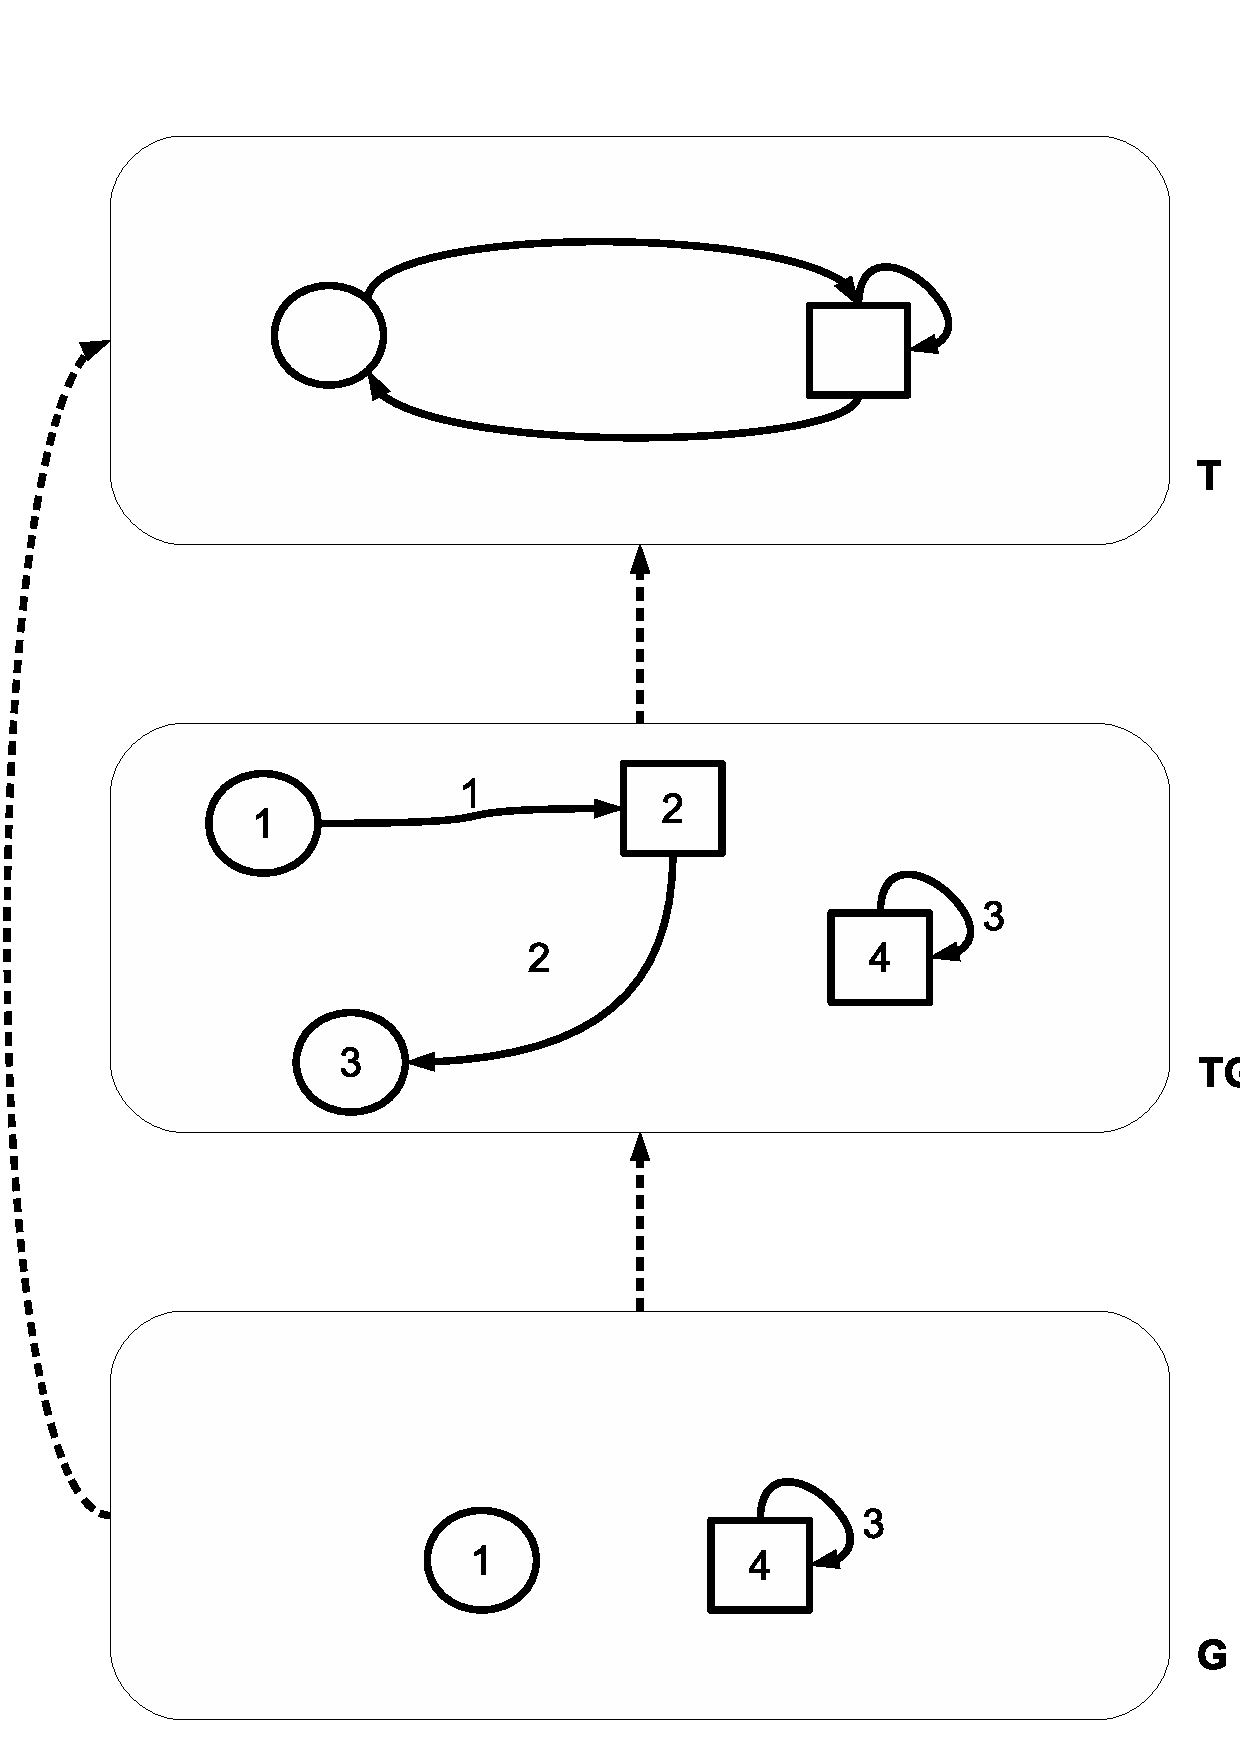
\includegraphics[scale=0.5]{images/process/doubly-typed-graph-example}}
  \caption{Doubly-typed graph}\label{fig:process:doubly-typed-graph}
\end{figure}

\end{example}

\begin{definition}[Doubly-Typed Graph Morphism]
  Given two doubly-typed graphs $G^{TG^T}$ and $H^{TG^T}$ and a graph morphism $g^T : G^T \rightarrow H^T$, we say that $g^T$ is a \emph{$TG^T$-doubly-typed graph morphism} if the following diagram commutes:

\diagram{
  G\ar[rr]^{g}\ar[dr]_{t^{G}}& & H\ar[dl]^{t^{H}} \\
   & TG\ar[d]^{type_{TG}} & \\
  & T &
}
\end{definition}

Notice that the (single) type morphisms $type_G : G \rightarrow T$ and $type_H : H \rightarrow T$ can be obtained respectively as $type_{TG} \circ t^G$ and $type_{TG} \circ t^H$.

\begin{example}[Doubly-Typed Graph Morphism Example] Figure~\ref{fig:process:doubly-typed-graph-morphism} shows a doubly-typed graph morphism $f : G^{TG^T} \rightarrow H^{TG^T}$.

\begin{figure}[!ht]
  \centering
  \fbox{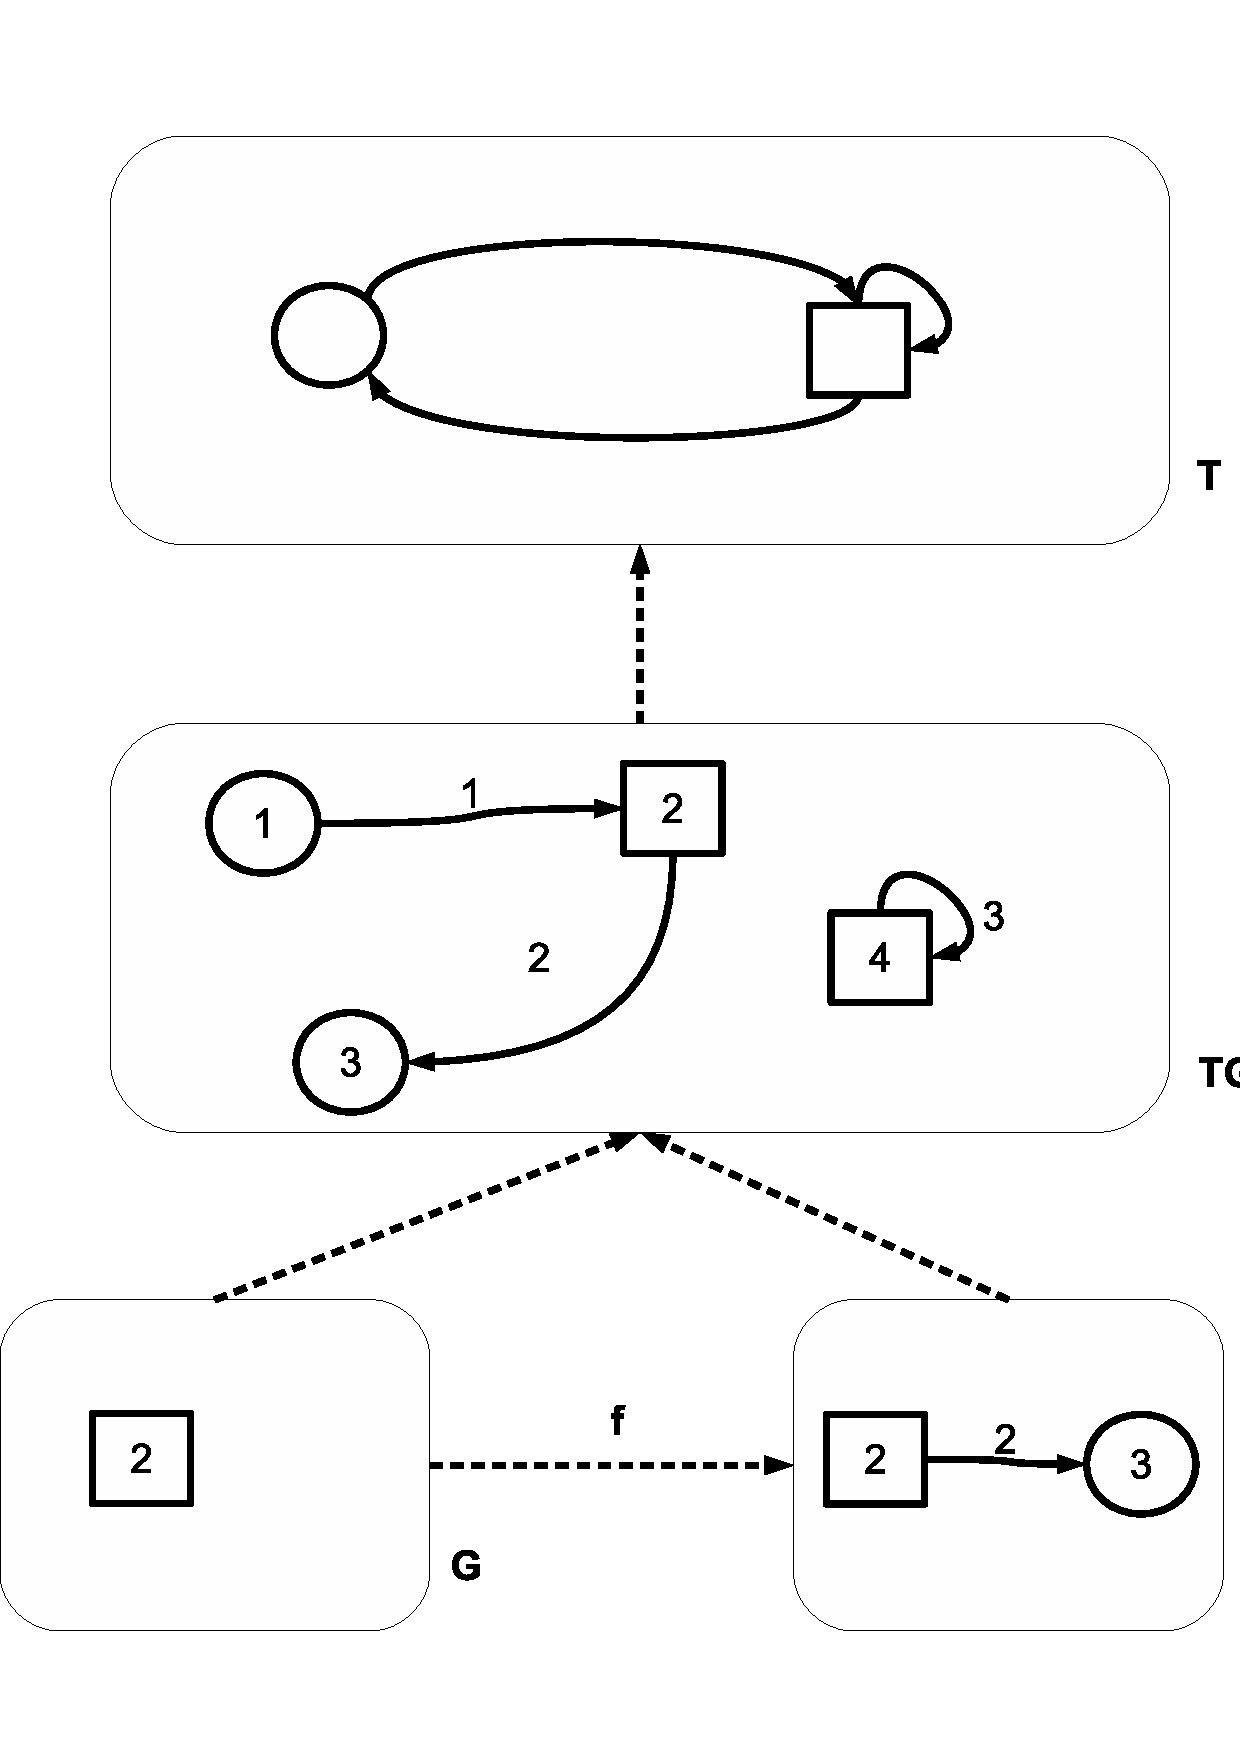
\includegraphics[scale=0.5]{images/process/doubly-typed-graph-morphism-example}}
  \caption{Doubly-typed graph morphism}\label{fig:process:doubly-typed-graph-morphism}
\end{figure}
\end{example}

\begin{remark} \cite{Ribeiro1996} defined different kinds of doubly-typed graph morphisms based on whether the doubly-type graphs and the type graphs are not the same. In this work we are only interested in the case where all doubly-typed graphs share the same double-type and type graphs. Therefore we will call the \mbox{\emph{$TG^T$-doubly-typed graph morphisms}} simply by \emph{doubly-typed graph morphisms} through the rest of this thesis.

\end{remark}


\begin{definition}[Doubly-Typed Graph Rule] A doubly-typed graph rule \doublyTypedRule{} is a span of injective doubly-typed graph morphisms $l : K \rightarrow L$ and $r : K \rightarrow R$.

\diagram{
  L\ar[dr] & K\ar[l]\ar[r]\ar[d] & R\ar[dl]\\
    & TG\ar[d] & \\
    & T &
}

  Given a doubly-typed graph rule \doublyTypedRule{}, its inverse rule is defined by \inverseDoublyTypedRule{}.

  Let the double-typing morphisms from $L^{TG^T}$, $K^{TG^T}$ and $R^{TG^T}$ be $t^{L^T}$, $t^{K^T}$ and $t^{R^T}$, respectively. For a rule $a = p^{TG^T}$ we call:

  \begin{itemize}
    \item $L_a = L_T$, $K_a = K_R$ and $R_a = R_T$, the left, gluing and right graphs of $a$.
    \item $pre_a = t^{L^T} : L^T \rightarrow TG^T$, the \emph{pre-condition} of the $a$.
    \item $post_a = t^{R^T} : R^T \rightarrow TG^T$, the \emph{post-condition} of $a$.
    %\item $r_a = r^T$, the \emph{rule pattern} of $a$.\tinytodo{Not sure if we will need the rule pattern.}
  \end{itemize}

\end{definition}

\begin{example}[Doubly-Typed Graph Rule Example]Figure~\ref{fig:process:doubly-typed-graph-rule} shows a doubly-typed graph rule which deletes an edge $\curvearrowleft_1$ and a node $\Circle_1$, preserves a $\Square_2$ and creates a node $\Circle_3$ and an edge $\curvearrowleft_2$.

\begin{figure}[!ht]
  \centering
  \fbox{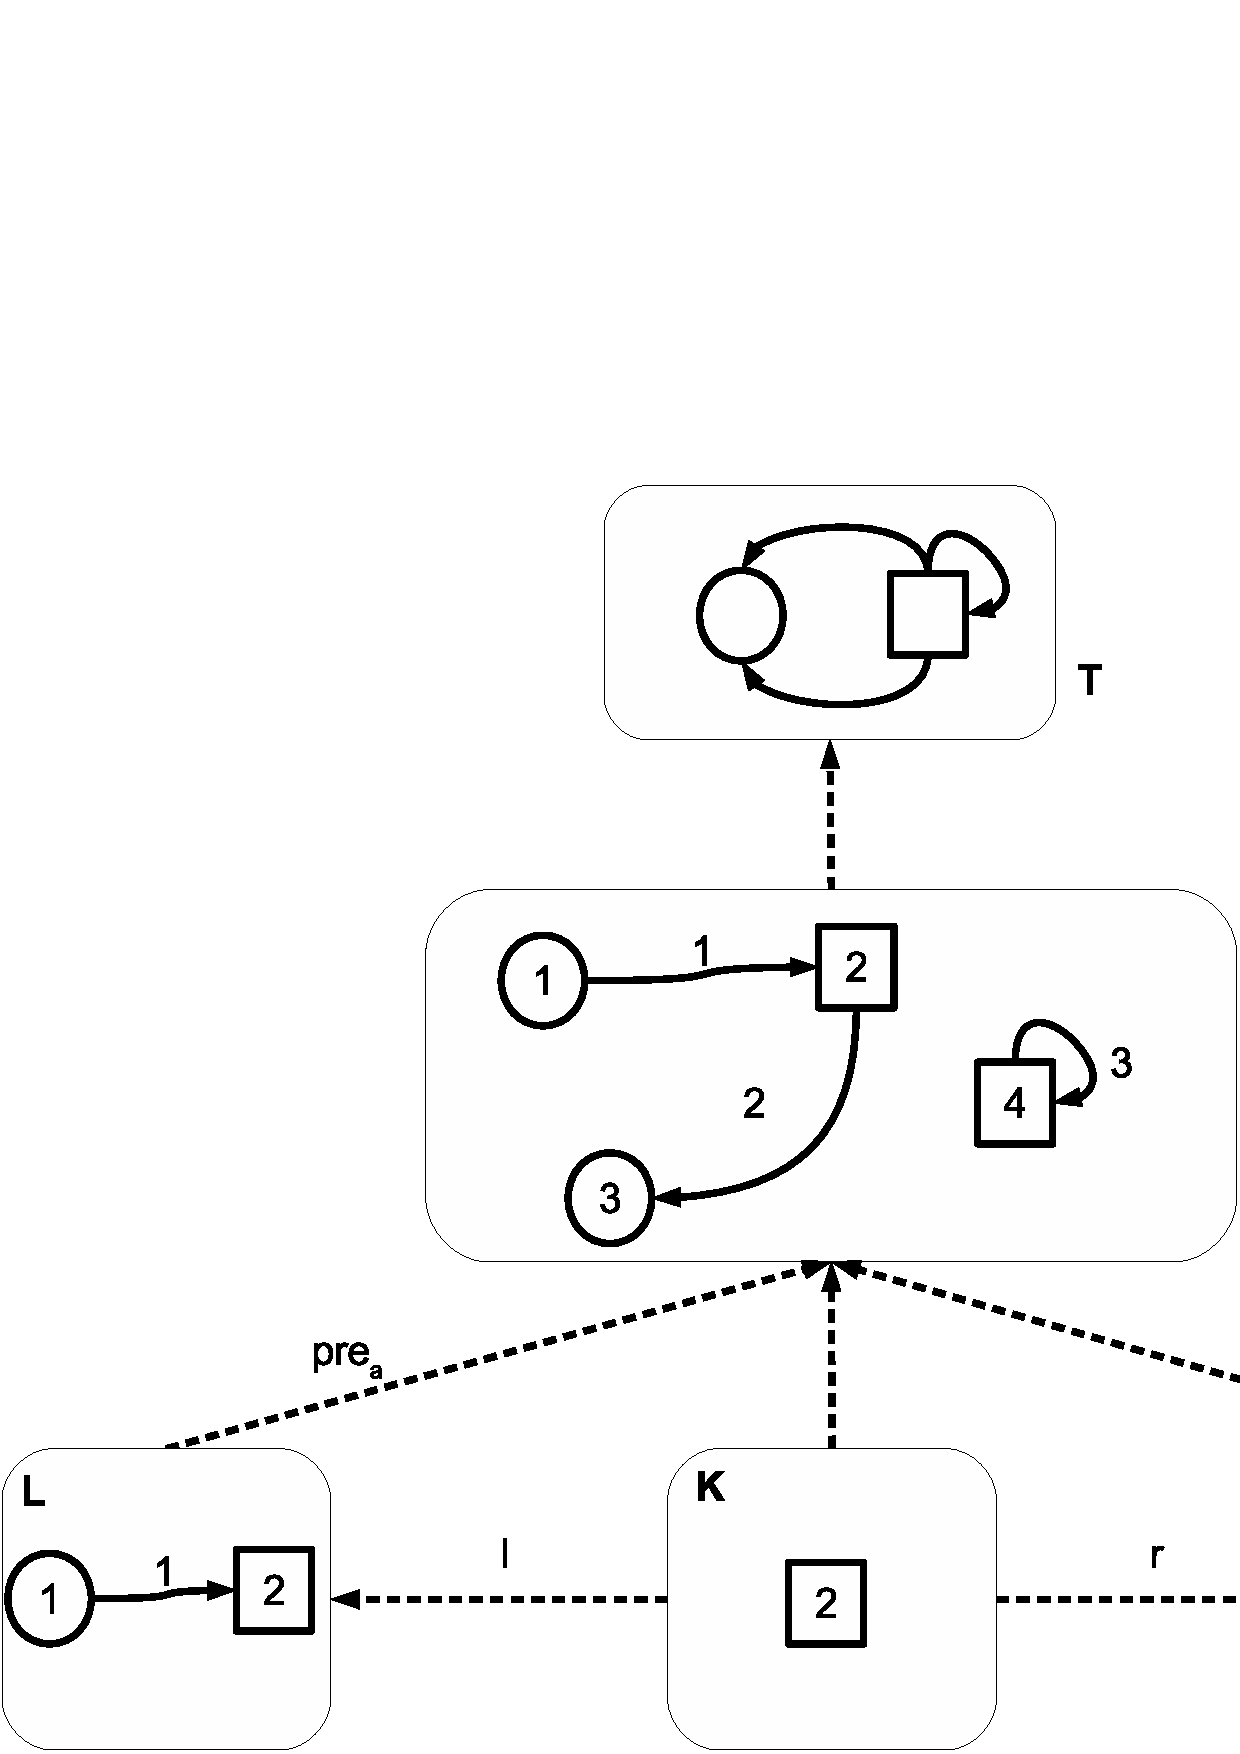
\includegraphics[scale=0.5]{images/process/doubly-typed-graph-rule-example}}
  \caption{Doubly-typed graph rule}\label{fig:process:doubly-typed-graph-rule}
\end{figure}
\end{example}

\begin{definition}[Negative Application Conditions on Doubly-Typed Graph Rules] A \emph{left} negative application condition over a doubly-typed graph rule $p^{TG^T}$ is of the form $NAC(n^T)$, where $n^T : L^T \rightarrow N^T$ is an arbitrary (single-)typed graph morphism. 
 
A (doubly-typed) match morphism $m^{TG^T} : L^{TG^T} \rightarrow G^{TG^T}$ of a rule $p^{TG^T}$ satisfies $NAC(n^T)$ on $L^{TG^T}$, written \mbox{$m^T \models NAC(n^T)$}, iff $\nexists$ $q^T : N^T \rightarrow G^T$ where $q^T$ injective and $q^T \circ n^T = m^T$.

\diagram{
  T & TG\ar[l]\\
  N\ar[u]\ar@{.>}[dr]|{|}_{q} & L\ar[u]\ar[d]^{m}\ar[l]_{n}\\
   & G\ar@/_2.1pc/[uu]
}

  A match $m^{TG^T} : L^{TG^T} \rightarrow G^{TG^T}$ satisfies a set \mbox{$NAC_L = \{NAC\left(n^T_i\right)|i \in I\}$} of left $NACs$, iff \mbox{$m \models NAC\left(n^T_i\right)$} $\forall i \in I$.

\emph{Right} negative application conditions are defined analogously for the right hand side of a rule and its comatch.
\end{definition}

\begin{remark}
We could have defined NACs whose morphisms are doubly-typed graph morphisms (which would then act specifically over doubly-typed graphs), but we will not use this kind of NACs later in our work. Therefore, we will use \emph{single-typed} NACs as the only NAC type in all of our \emph{doubly-typed graph grammars}, and $NAC(n)$ as a synonym of $NAC(n^T)$.

\end{remark}

\newadd{In a grammar whithout NACs, if there is a sequence of graph transformations $t_0\ldots t_n$ where all pairs $(t_i,t_j)$ of transformations are sequentially independent, then it is possible to \emph{switch} the
order of application for any pair in that sequence and still achieve the same final result (up to isomorphism). However, this is not always true when the grammar has NACs~\cite{Corradini2013}.} When dealing with the classical notion of NACs, there may be situations where the NAC of a rule can be triggered by the cumulative effect of applying two (or more) other rules, while the same rules would not trigger this NAC without the other. This may lead to a situation where conflicts and dependencies
are not stable under switch. An example is shown in Figure~\ref{ex:process:instability}.

\begin{example}[Instability of Conflicts and Dependencies]\label{ex:process:instability}The rules depicted in Figure~\ref{fig:process:instability} show a situation where the independency between rules is not stable under switch equivalence.

  In this example, all rules are independent and also do not conflict with each other in the sense of Definitions~\ref{def:classic-dependency} and~\ref{def:classic-conflict}. Thus, in theory, it should be possible to apply this rules in any order or in parallel. Particularly, it is possible to apply all rules in the order they appear in the figure, i.e. $[p_1, p_2, p_3]$. It is also possible to apply them in the orders $[p_1, p_3, p_2]$, $[p_2, p_1, p_3]$ and $[p_3, p_1, p_2]$. However, the
  sequences $[p_2, p_3, p_1]$ or $[p_3, p_2, p_1]$ are not possible. This problem arises from the fact that $p_2$ and $p_3$ independently create a piece of the pattern forbidden by the NAC of $p_1$ in a way that, although the effects of each rule by itself does not trigger the NAC of $p_1$, their combined effects do.

\begin{figure}[!ht]
  \centering
  \fbox{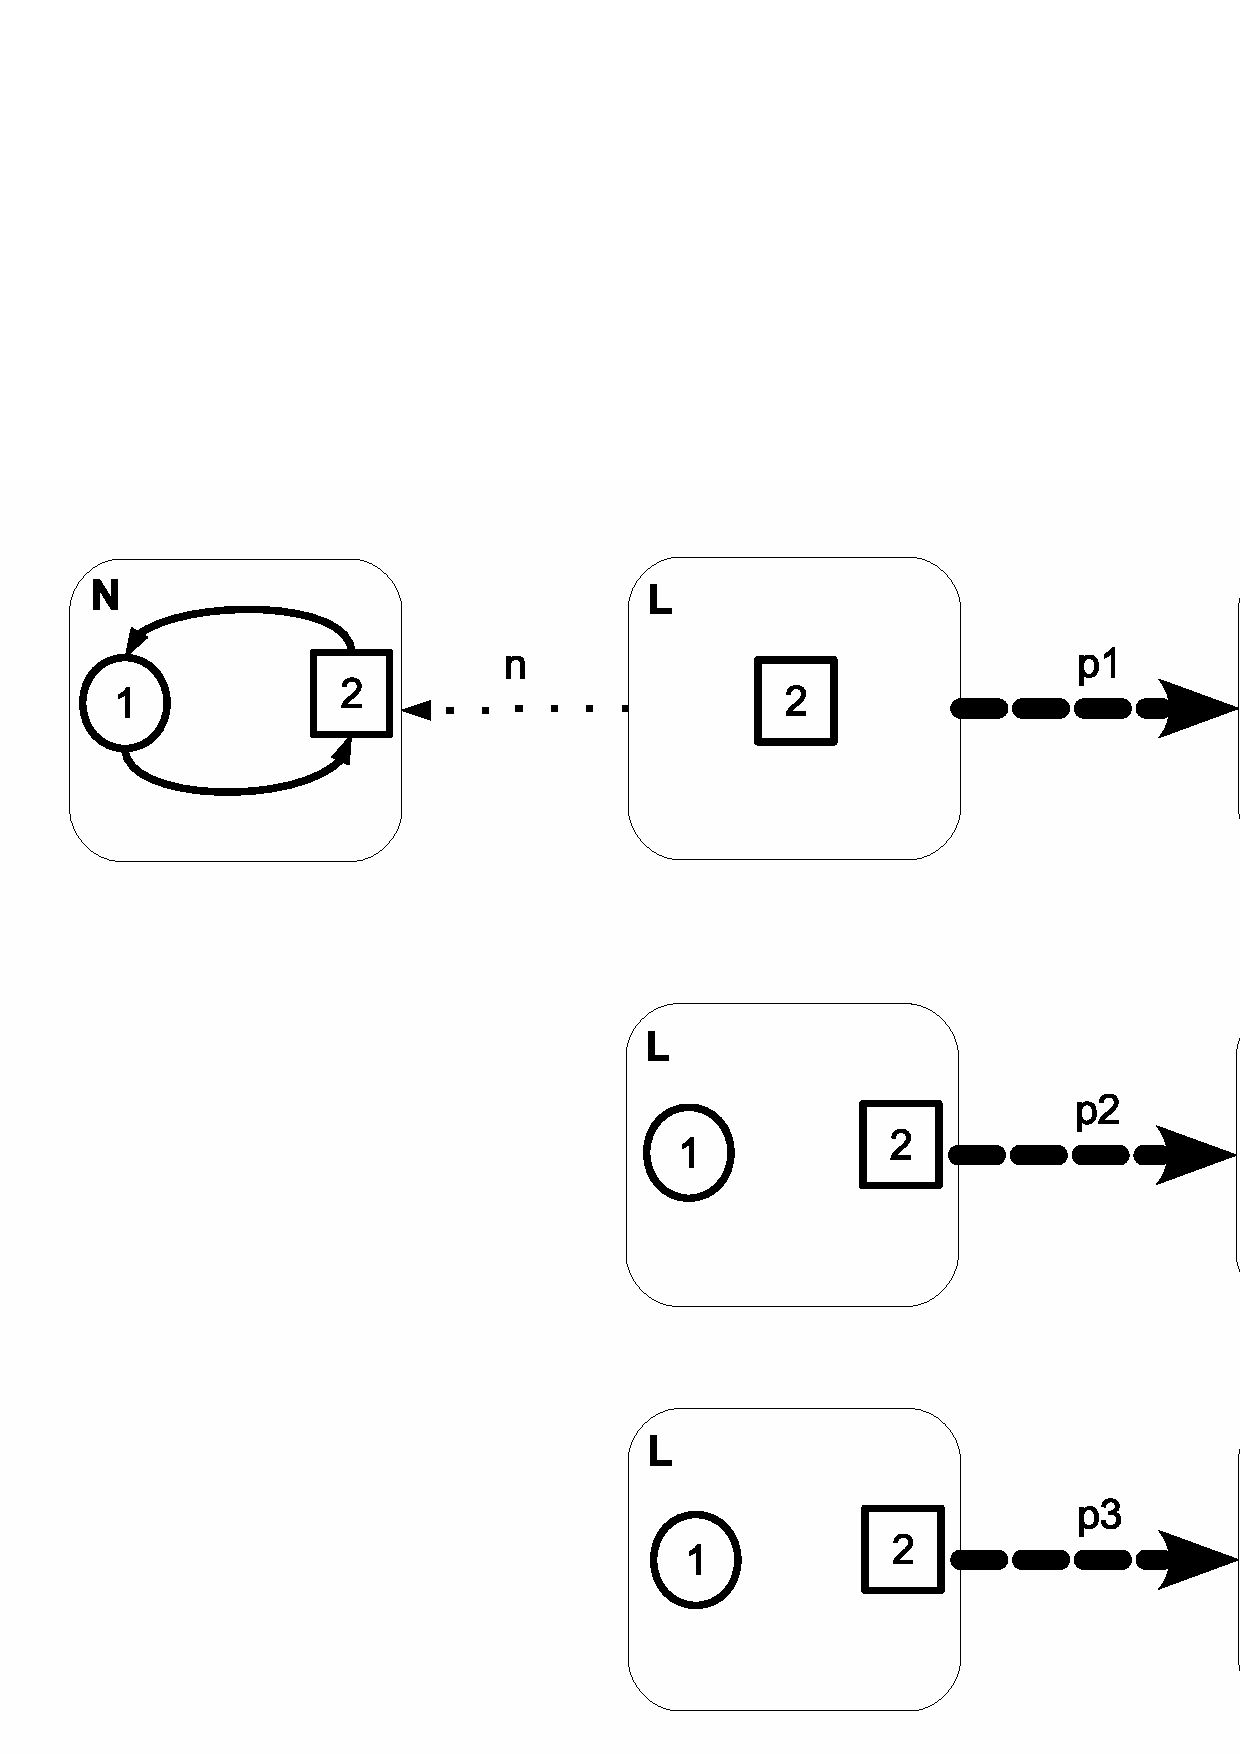
\includegraphics[scale=0.5]{images/process/instability-example}}
  \caption{Instability of conflicts under shift\\}\label{fig:process:instability}
\end{figure}

\end{example}

As we are interested in constructing a canonical representation of several possible derivations for a set of rules of a grammar, we will make use of a special type of NACs called \emph{incremental NACs}.

\emph{Incremental NACs}, originally defined in~\cite{Corradini2013} and~\cite{Corradini2014}, have the property of extending the forbidden context of a match by a single edge or a single node. Thus, each NAC forbids only one element at a time and therefore there is no possible way to trigger a NAC by the cumulative effect of more than one rule.

\begin{definition}[Incremental NACs] Given a monomorphism \mbox{$n : L \rightarrow N$}, $NAC(n)$ is said to be incremental if for any possible pair of decompositions \mbox{$g_1 : L \rightarrow O_g;g_2 : O_g \rightarrow N$} and \mbox{$f_1 : L \rightarrow O_f;f_2 : O_f \rightarrow N$} as in the diagram below, where all morphisms are monos and \mbox{$f_1;f_2 = n = g_1;g_2$}, there exists a mediating morphism $o_1 : O_g \rightarrow O_f$ or $o_2 : O_f \rightarrow O_g$, such that the resulting triangles
  commutes.

\diagram{
  & O_g\ar[dr]^{g_2}\ar@{.>}@/_0.5pc/[dd]|<<<<<<{o_1} &  \\
  L\ar[ur]^{g_1}\ar[dr]_{f_1}\ar[rr]|<<<<{n}&     & N\\
    & O_f\ar[ur]_{f_2}\ar@{.>}@/_0.5pc/[uu]|<<<<<<<<{o_2} & 
}

\end{definition}

\begin{example}[Incremental NACs]Figure~\ref{fig:process:incremental-nacs} shows all possible formats that any valid incremental NAC can assume.

\begin{figure}[!ht]
  \centering
  \fbox{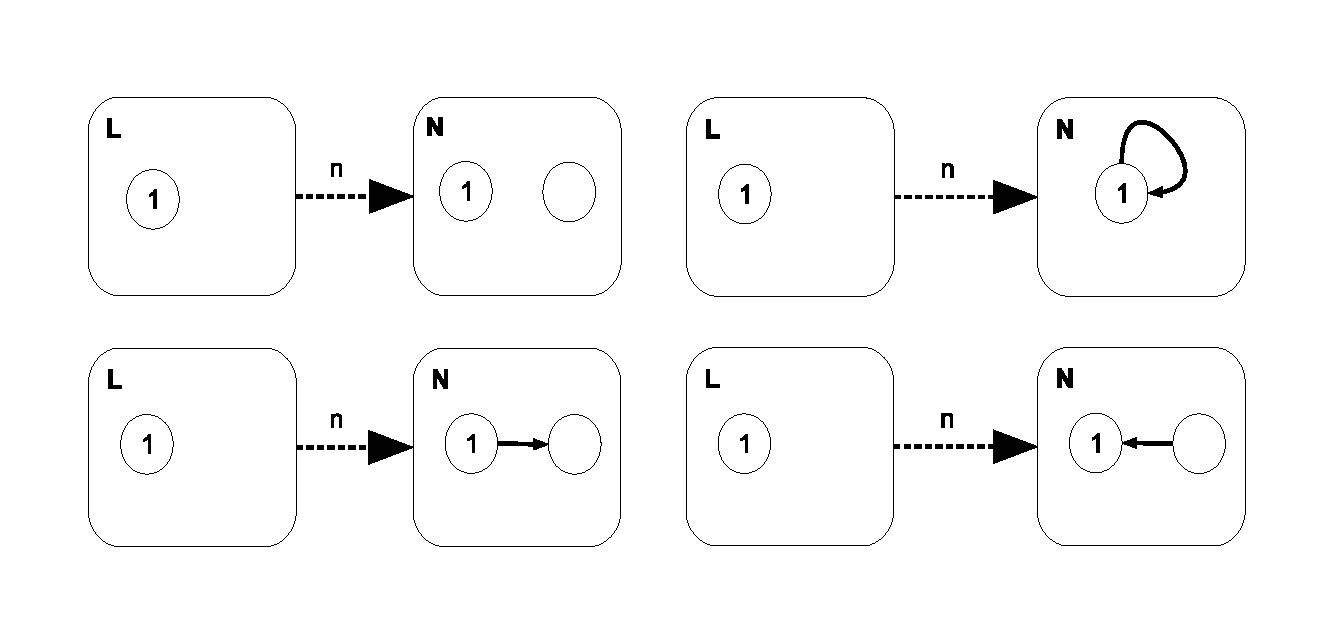
\includegraphics[scale=0.7]{images/process/incremental-nacs}}
  \caption{Canonical Incremental NACs}\label{fig:process:incremental-nacs}
\end{figure}
\end{example}

At first, it may seem that we are loosing expressive power by restricting the NACs we use in our grammars to incremental NACs only, however ~\cite{Corradini2013} has shown two important results regarding that. First, they showed that incremental NACs are sufficient to model most of real applications using $GTS$s. Second, they presented an algorithm to compile rules with general NACs to rules with incremental NACs only, generating a new $GTS$ that is able to simulate the original one.

\begin{definition}[Triggering element] Given a rule \graphrule{} with an incremental, non trivially triggered NAC \nac{}, and a monomorphic match \match{}, where there is an injective $q : N \rightarrow G$, therefore $m \not\models NAC(n)$. There is exactly one element that will complete the match towards triggering the NAC, this element is present in the difference between the images of $q$ and $m$.

  Let $G_{|N}$ be the image of $q$ and $G_{|L}$ the image of $m$, and \mbox{$T = G_{|N} - G_{|L}$}.\footnote{In this case, $T$ may not be a graph, we are here abusing the notation and treating $T$ as a set $V$ of vertices and a set $E$ of edges.} The triggering element of this NAC is:

  \begin{itemize}
    \item $x \in E(T)$, if $E(T) \neq \varnothing$;
    \item $x \in V(T)$ otherwise.
  \end{itemize} 
\end{definition}

\begin{example}[Triggering Element]
Since incremental NACs extend the match by forbidding only one element at a time, this element can be easily identified when looking at the instance graph: it corresponds to the element which is not mapped by the morphism $n$ from the NAC to the instance graph.\tinytodo{Prepare example}
\end{example}

\begin{definition}[Doubly-Typed Graph Grammars] A \emph{doubly-typed graph grammar} is a tuple $GG = \left(TG^T, I^{TG^T},P \right)$ where $TG^T$ is the double-type graph of the grammar, $I^{TG^T}$ is a doubly-typed graph, called the \emph{initial graph} of the grammar and $P$ is a set of doubly-typed graph rules.
\end{definition}

\begin{definition}[Core Graph]\label{def:core-graph} Given a doubly-typed graph grammar \doublyTypedGraphGrammarCore{}, we have that \coreGraph{} is a \emph{core graph} iff the following two conditions hold:

\begin{enumerate}

\item \mbox{$\forall x \in$ \coreGraph $: \exists! y \in (I^T \uplus (\uplus_{i \in P} (R_i - K_i))$}:
\[ x =
    \begin{cases}
      in_{GG}\parens{y},$ if $y \in I^T\\
      post_i(y),$ if $y \in R_i - K_i\\
    \end{cases}
   \]

\item \mbox{$\forall x \in$ \coreGraph $: \exists^{\leq1} y \in \uplus_{i \in P} (L_i - K_i)$}:
\[ x =
    \begin{cases}
      pre_i(y),$ if $y \in L_i - K_i\\
    \end{cases}
   \]\end{enumerate}

  The first condition assures that every element in the \emph{core graph} was either already present in the initial graph or was created by one and only one rule. The second condition assures that for every element that is deleted, it is deleted only once by only one rule. \important{the second condition is valid only for deterministic executions, see how this goes after reestructring the text}
\end{definition}

The idea is that each element within a \emph{core graph} has a unique origin. At the same time, the \emph{core graph} contains all elements necessary (created, deleted and preserved) by all rules in its underlying grammar.

\begin{example}[Doubly-Typed Graph Grammar and Core Graph Example] \mbox{Figure~\ref{fig:process:core-graph:counter-example}} shows a doubly-typed graph grammar, whose double-type is not a core graph. That happens because $\Square_2$ is created by both rules $p_1$ and $p_2$, as well as $\Circle_1$ is deleted by both $p_2$ and $p_3$.

  On the other hand, Figure~\ref{fig:process:core-graph:example} shows a doubly-typed graph grammar whose double-type is also a core graph: all elements are either created only once or, if not created by any rule, are present in the initial graph: $\Square_2$ and $\curvearrowleft_1$ are created by $p_1$, $\curvearrowleft_3$ by $p_2$, $\Circle_3$ and $\curvearrowleft_2$ by $p_3$ and $\Circle_1$ is present on the initial graph. Also, the deleted elements are deleted only once: $\Circle_1$ and
  $\curvearrowleft_1$ by $p_3$.

  It is important to notice that, even though the $TG$ graphs in both grammars are isomorphic, only the one in Figure~\ref{fig:process:core-graph:example} is a core graph. This can be explained by looking to their underlying grammars (initial graphs and rules), where one of them satisfies the conditions presented in Definition~\ref{def:core-graph} and the other not.
\begin{figure}[!ht]
  \centering
  \begin{subfigure}[t]{.5\textwidth}
    \centerline{\fbox{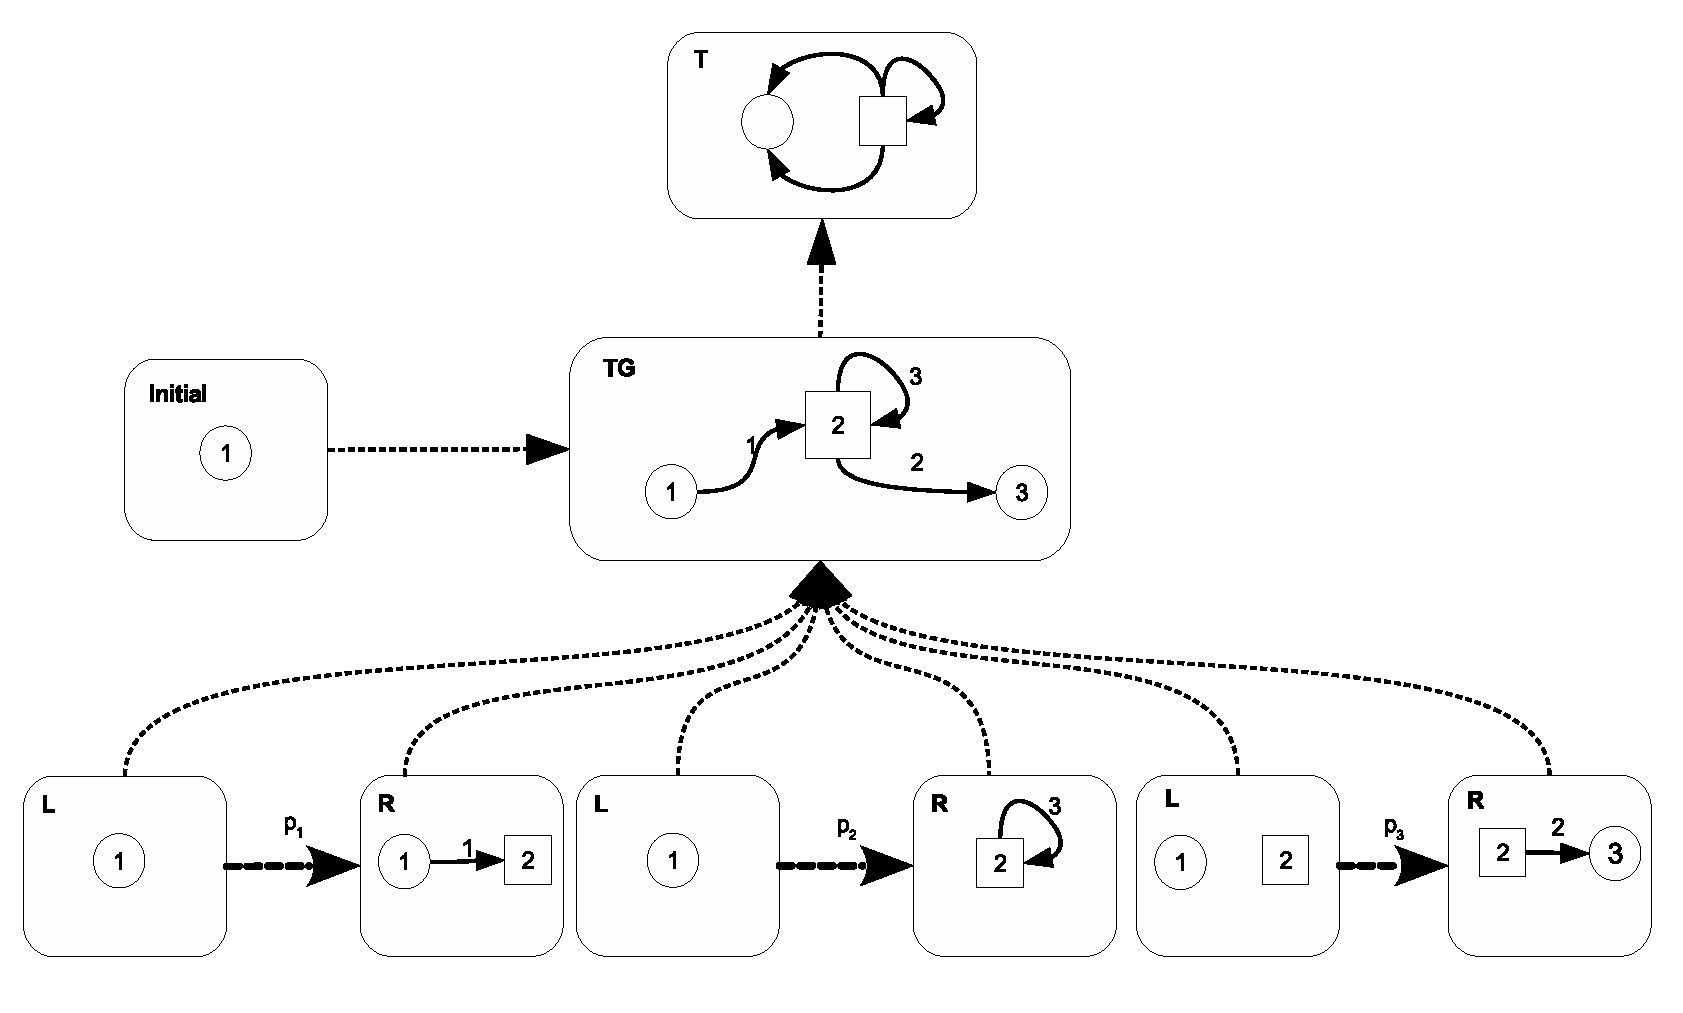
\includegraphics[scale=0.5]{images/process/core_graph/counter_example}}}
    \caption{A grammar with a double-type graph that is not a core graph.}\label{fig:process:core-graph:counter-example}
  \end{subfigure}
  \begin{subfigure}[t]{.5\textwidth}
    \centerline{\fbox{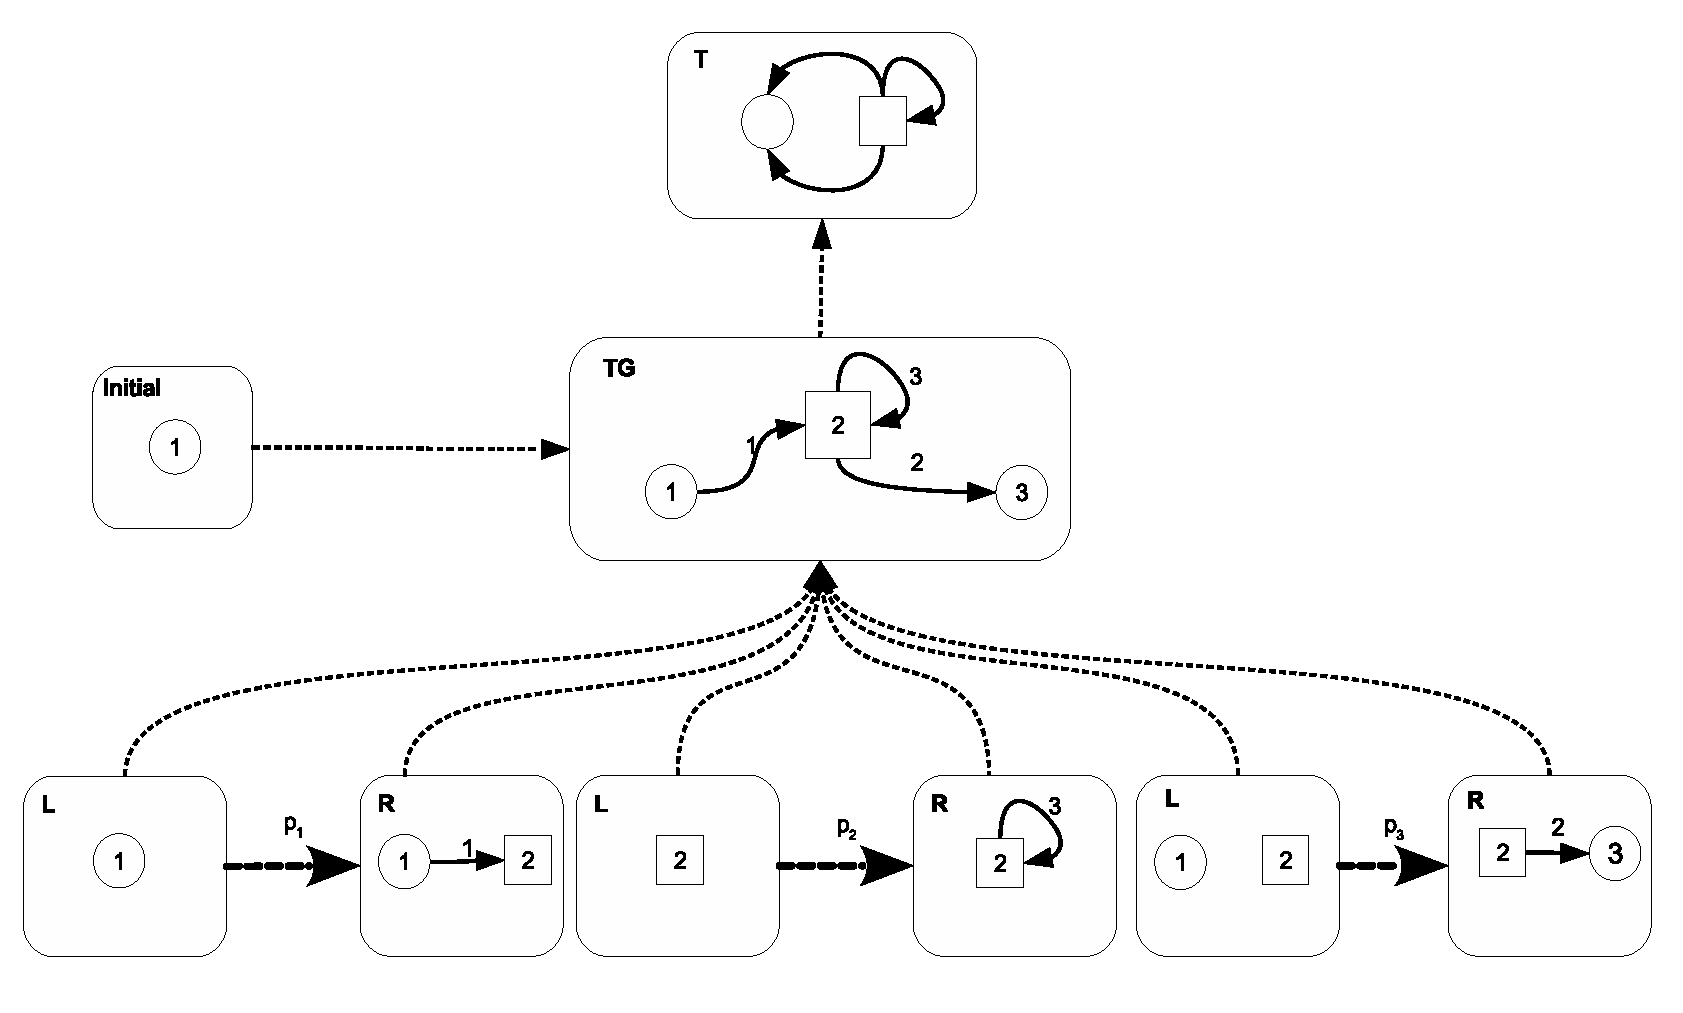
\includegraphics[scale=0.5]{images/process/core_graph/example}}}
    \caption{A grammar with a double-type graph that is also a core graph.}\label{fig:process:core-graph:example}
  \end{subfigure}

  \caption{Doubly-typed graph grammars}\label{fig:process:doubly-typed-grammars}
\end{figure}

\end{example}

\begin{notation}[Restriction to Image] Given an arbitrary morphism $f : A \rightarrow X$, we will denote as $f' : A \rightarrow X_{|A}$ the morphism derived from $f$ where $X_{|A}$ is the image of $f$.

  For two arbitrary morphisms $f : A \rightarrow X$ and $g : B \rightarrow X$, we will denote as $f' : A \rightarrow X_{|AB}$ and $g' : B \rightarrow X_{|AB}$ the morphisms derived from $f$ and $g$ where $X_{|AB}$ is the joint image of both $f$ and $g$. \important{As a result, $X_{|AB}$ contains all and only the elements of $X$ that are mapped from $A$ or $B$ to $X$, preserving the original mappings?}
\end{notation}

\begin{definition}[Strongly Safe (Doubly-Typed) Graph Grammars] Given \doublyTypedGraphGrammarCore{} a doubly-typed graph grammar, $GG$ is said to be \emph{strongly safe} if its double-type graph is also a core graph.

  Each rule in a strongly safe graph grammar is also called an \emph{action}. We say that an action $a$ creates an element $e$ iff $e \in R(a) - K(a)$. Similarly, $a$ deletes $e$ iff \mbox{$e \in L(a) - K(a)$}. Finally, if $e$ is present in $K(a)$, we say that $a$ preserves $e$. 

When dealing with actions, we will use a slightly different interpretation for the graph transformations: 
  
\begin{itemize} 
  \item Actions are always applied over the core graph: the match of an action is equal to its pre-condition $pre_a : L \rightarrow C^T$, as well as the comatch is equal to its post-condition $post_a : R \rightarrow C^T$.

  \item Given an action \action{} with NACs and its application over the core graph, we restrict the search for the injective morphism $q : N \rightarrow C^T$ to the image of the match $q : N \rightarrow C^T_{|L_a}$ (comatch $q : N \rightarrow C^T_{|R_a}$) rather than the entire core graph. Similarly, when searching for conflicts or dependencies within two actions $a_1, a_2$ with NACs, the test of NAC satisfiability performed on the overlapping between the actions is restricted to the joint image of the respective morphisms in the core graph.
\end{itemize}

  \important{review these two following paragraph, leila did not understand:}

  \important{also, review the nac application, it may only make sense for conflicts / dependencies, not for an isolated action}
  
  \uline{The ``restricted to the image'' search is meant to avoid the triggering of NACs by elements that are present in the core graph, therefore present in the match/comatch, but that do not exist when looking only at the actions interacting at the moment. It also avoids the dangling condition in the core graph out of the scope of the actions.}
  
  \uline{This restriction together with the use of incremental NACs allow us to locally compute the conflicts and dependencies for each pair of actions, without having to be concerned about global effects of other actions coming into play.}



\end{definition}

\begin{remark}[Strongly Safe Grammars] Throughout this work, we will use only strongly safe grammars whose set $P$ of actions is finite and each action in $P$ is distinct from the others.

\end{remark}

\begin{example}[Strongly Safe Graph Grammar] Figure~\ref{fig:process:core-graph:example} also depicts a strongly safe graph grammar as the double-type graph of the grammar is, in fact, a core graph.
\end{example}

\section{Relations within Strongly Safe Graph Grammars without NACs}

Given a strongly safe graph grammar, its core graph contains all elements used (created, read or deleted) during one possible execution of the grammar. Moreover, as each element has a unique origin, the core graph can be considered to contain the entire ``execution history'' of its underlying grammar.

We are here interested in some of the properties that can be found by looking at this history. Particularly, which kind of relations exist among actions and elements, whether it is possible to find sequences in which all actions are applied and which graphs can be considered valid (reachable) by this grammar.

In~\cite{Ribeiro1996}, causal, conflict and occurrence relations for strongly safe graph grammars were defined. There, the graph transformation approach used was the \emph{Single Pushout} (SPO) without NACs.

\cite{Corradini1996} also defined a different notion of causal relation, equivalent to the occurrence relation in the previous mentioned work, with respect to the DPO approach without NACs.

Both authors use these relations to find out whether all the actions of a strongly safe graph grammar are applicable and prove the above mentioned properties about them. However, these relations alone are not sufficient for our purpose when the actions may have NACs.

Here we recall these definitions, which correspond to the \emph{existential relation} and the \emph{unconditional causal dependency and conflict relations} defined in the following, and extend them to create an equivalent notion of \emph{conditional relations} that work for grammars in the DPO approach with NACs.

\begin{definition}[Existential Relation] This is the \emph{causal relation} defined in \cite{Corradini1996} for the DPO approach without NACs. Given  \doublyTypedGraphGrammarCore{} a strongly safe graph grammar, actions \mbox{$a_1, a_2 \in P, a_1 \ne a_2$} and an element \mbox{$e_1 \in N(C^T) \cup E(C^T)$}, then:

  \begin{enumerate}
    \item If $a_1$ deletes $e_1$, then $e_1 <_e a_1$.
    \item If $a_1$ creates $e_1$, then $a_1 <_e e_1$.
    \item If $a_1$ creates $e_1$ and $a_2$ preserves $e_1$, then $a_1 <_e a_2$.
    \item If $a_1$ preserves $e_1$ and $a_2$ deletes $e_1$, then $a_1 <_e a_2$. 
    \item The \emph{existential relation} $\leq_e$ of $P \cup N(C^T) \cup E(C^T)$ is the reflexive and transitive closure of $<_e$.
  \end{enumerate}
\end{definition}

This relation represents restrictions over creation, use (preservation) and deletion of elements by actions that are used to characterize executions of the underlying rules. We have that an action $a$ must occur after all the actions that create the elements on which it depends. Analogously, $a$ must occur before all actions that delete the elements created/preserved by $a$.

In \cite{Corradini1996} it is shown that if this relation is a \emph{partial order}, then any total order with respect to it is a sequentialization in which all productions of the underlying grammar are applicable. However, this condition is not sufficient in grammars whose rules may be equipped with NACs, as shown in example~\ref{ex:process:existential-relation-fail}.

\begin{example}[Existencial Relation in Grammars without NACs]\label{ex:process:existential-relation} Given the strongly safe grammar corresponding to the core and initial graphs in Figure~\ref{fig:process:existential-relation:core-graph} and the set of rules in Figure~\ref{fig:process:existential-relation:example}, we have that:

\begin{itemize}
  \item $a_1 <_e \triangle_2$
  \item $a_2 <_e \Square_1$ and $a_2 <_e$ $\curvearrowleft_1$
  \item $a_3 <_e$ $\curvearrowleft_2$
  \item $a_2 <_e a_1$ by creation/preservation of $\Square_1$
\end{itemize}

  The existential relation for this grammar is (without the pairs due to reflexivity): $a_1 \leq_e \triangle_2$, $a_2 \leq_e \Square_1$, $a_2 \leq_e$ $\curvearrowleft_1$, $a_3 \leq_e$ $\curvearrowleft_2$, $a_2 \leq_e a_1$, $a_2 \leq_e \triangle_2$. Notice that the only pair in this relation where both elements are actions is \mbox{$a_2 \leq a_1$}, therefore, we have that all actions in this grammar can be applied as long as $a_2$ is applied before $a_1$ ($a_2$ crates the element $\Square_1$
  which is necessary for $a_1$ to be applied). In particular, the following sequences of actions are valid and lead to the same result: $[a_2,a_1,a_3],[a_2,a_3,a_1],[a_3,a_2,a_1]$.

\begin{figure}[!ht]
  \centering
  \begin{subfigure}[t]{.5\textwidth}
    \centerline{\fbox{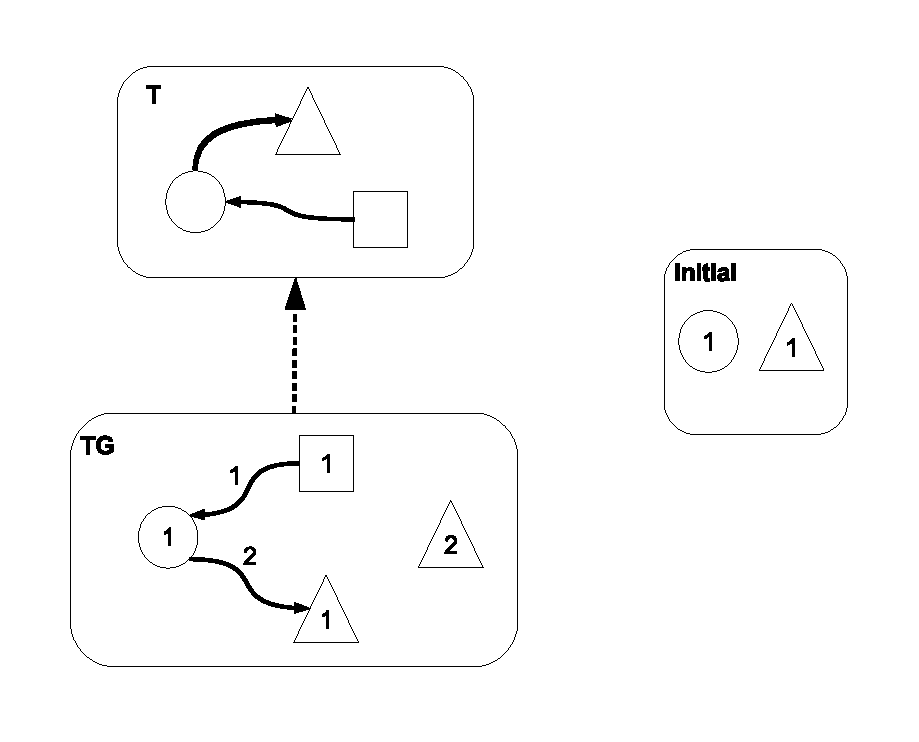
\includegraphics[scale=0.6]{images/process/existential-relation/core-graph}}}
    \caption{Core and initial graphs}\label{fig:process:existential-relation:core-graph}
  \end{subfigure}
  \begin{subfigure}[t]{.5\textwidth}
    \centerline{\fbox{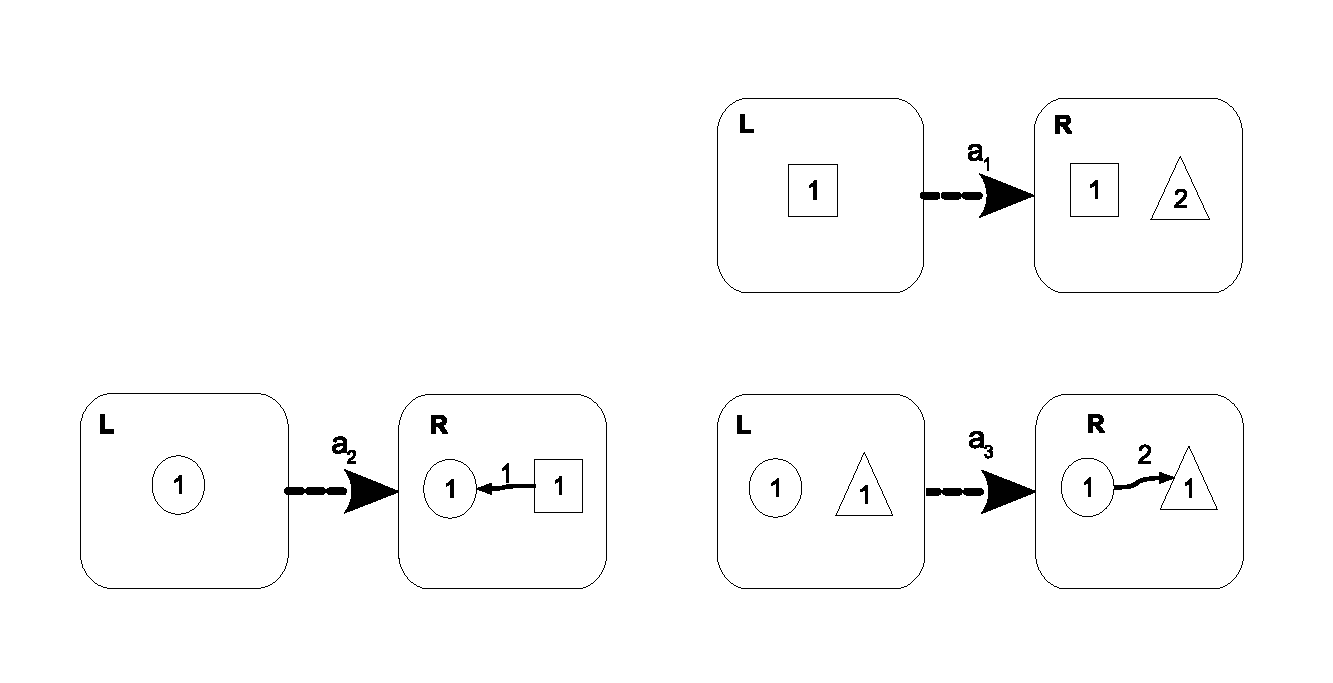
\includegraphics[scale=0.6]{images/process/existential-relation/example}}}
    \caption{A strongly safe grammar without NACs}\label{fig:process:existential-relation:example}
  \end{subfigure}
  \begin{subfigure}[t]{.5\textwidth}
    \centerline{\fbox{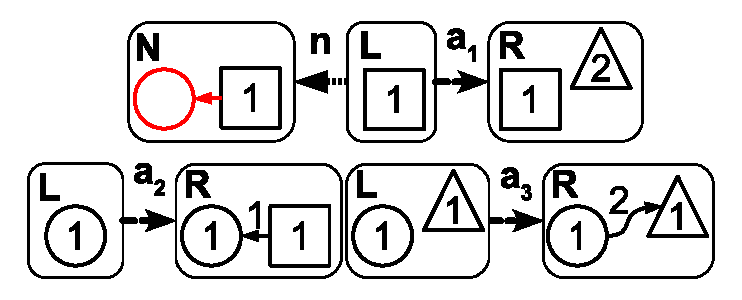
\includegraphics[scale=0.6]{images/process/existential-relation/example-nacs}}}
    \caption{A strongly safe grammar with NACs}\label{fig:process:existential-relation:example-nacs}
  \end{subfigure}
  \stepcounter{doubly-typed-grammar-counter}
  \caption{Strongly safe grammar GG\arabic{doubly-typed-grammar-counter}}\label{fig:process:existential-relation}
\end{figure}
\end{example}

The same definition can be attempted in a strongly safe grammar where actions are equipped with NACs. However, as shown in the next example, it lacks the same properties as in the context without NACs.

\begin{example}[Existential Relation in Grammars with NACs]\label{ex:process:existential-relation-fail}Consider the strongly safe grammar corresponding to the core and initial graphs in Figure~\ref{fig:process:existential-relation:core-graph} and the set of rules in Figure~\ref{fig:process:existential-relation:example-nacs}. 

  We have the same the same existential relation as the one presented in Example~\ref{ex:process:existential-relation}, since the structure of the actions is the same in both examples, except for the NAC in the action $a_1$ on Figure~\ref{fig:process:existential-relation:example-nacs}. In this example, we still have that $a_2$ must be applied first in order for $a_1$ to be applied. However, besides creating the $\Square_1$ needed for $a_1$, $a_2$ also creates a $\curvearrowleft_1$ from $\Square_1$ to $\Circle_1$ which is a pattern forbidden by the NAC on $a_1$. Therefore, we have that $a_2$ also causes a \emph{produce-forbid} conflict with $a_1$. Moreover, the only other action $a_3$ does not delete any element that could help undoing the forbidden pattern. Thus, there is no possible way of applying all actions of this grammar, even though the existential relation is a partial order.

\end{example}

\iffalse
The next \emph{unconditional relations} are equivalent to the \emph{causal dependency} and \emph{weak conflict} relations presented at~\cite{Ribeiro1996}, but for the DPO rather than the SPO approach. These relations will be used as basis to the \emph{conditional relations} that will be later defined for conflicts and dependencies with NACs.

Regarding both unconditional and conditional dependency relations, their definitions are based on the following intuition:

\begin{intuition} An action $a_1$ is a direct cause of an action $a_2$ if either $a_1$ creates some element that is needed by $a_2$ (unconditional causal dependency) or $a_1$ deletes an element that is both forbidden by a NAC of $a_2$ and existent before the application of $a_2$ (conditional causal dependency). In both cases, we have that $a_2$ can only happen after $a_1$ has been applied.
\end{intuition}

\begin{figure}[!ht]
  \centering
  \begin{subfigure}[t]{.5\textwidth}
    \centerline{\fbox{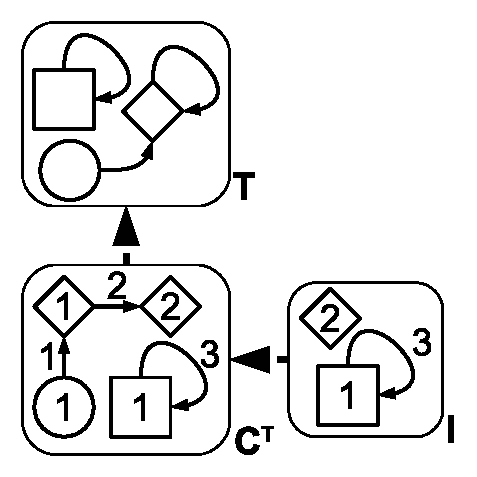
\includegraphics[scale=0.5]{images/process/unconditional-relation/core-graph}}}
    \caption{Core and initial graphs}\label{fig:process:unconditional-relation:core-graph}
  \end{subfigure}

  \begin{subfigure}[t]{.5\textwidth}
    \centerline{\fbox{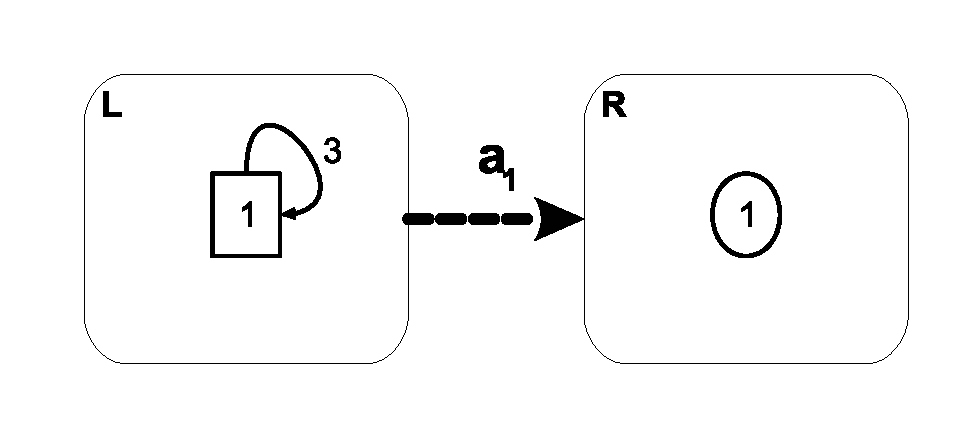
\includegraphics[scale=0.45]{images/process/unconditional-relation/a1}}}
    \caption{Action $a_1$}\label{fig:process:unconditional-relation:a1}
  \end{subfigure}%
  \begin{subfigure}[t]{.5\textwidth}
    \centerline{\fbox{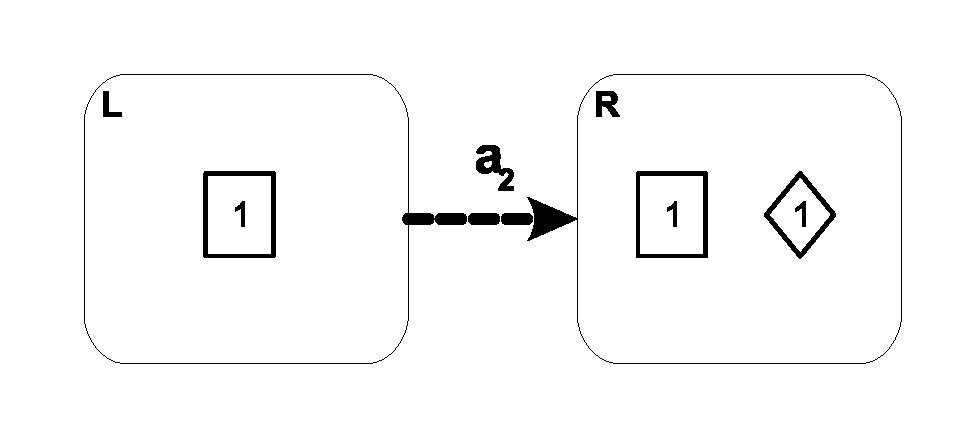
\includegraphics[scale=0.45]{images/process/unconditional-relation/a2}}}
    \caption{Action $a_2$}\label{fig:process:unconditional-relation:a2}
  \end{subfigure}

  \begin{subfigure}[t]{.5\textwidth}
    \centerline{\fbox{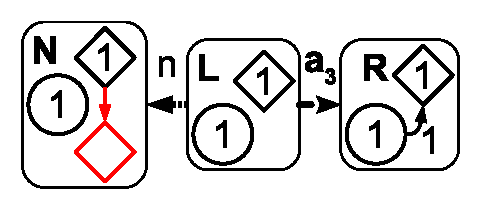
\includegraphics[scale=0.45]{images/process/unconditional-relation/a3}}}
    \caption{Action $a_3$}\label{fig:process:unconditional-relation:a3}
  \end{subfigure}%
  \begin{subfigure}[t]{.5\textwidth}
    \centerline{\fbox{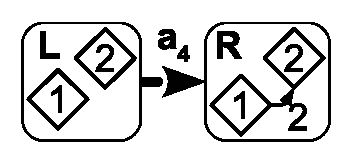
\includegraphics[scale=0.45]{images/process/unconditional-relation/a4}}}
    \caption{Action $a_4$}\label{fig:process:unconditional-relation:a4}
  \end{subfigure}
  \stepcounter{doubly-typed-grammar-counter}
  \caption{Strongly safe grammar GG\arabic{doubly-typed-grammar-counter}}\label{fig:process:unconditional-relation}
\end{figure}

\begin{definition}[Unconditional Causal Dependency Relation\footnote{Also called Produce-Use Relation.}]\label{def:unconditional-causal-dependency} Given \doublyTypedGraphGrammarCore{} a strongly safe graph grammar. Let $a_1, a_2 \in P$, $a_1 \ne a_2$, \mbox{$e_1, e_2 \in $ \coreGraph{}} and $e_1 \ne e_2$. Then: 

  \begin{enumerate}
    \item The action $a_2$ is \emph{directly causally dependent} on $a_1$, written $a_1 <_{pu} a_2$, iff \mbox{$\not\exists h_{21} : L_2 \rightarrow D_1$ s.t. \mbox{$d_1 \circ h_{21} = pre_2$}}, where the two squares are pushouts and $C^T_{|R_1L_2}$ ($C^T$ restricted to the joint image of $post_1$ and $pre_2$) satisfies the NACs for $a_2$ and $a_1^{-1}$.

\diagram{
   & & N_1^{-1} & & N_2 & & \\
      L_1 & K_1\ar[d]\ar[l]\ar[r] & R_1\ar[u]\ar[dr]_{post_1} & & L_2\ar[u]\ar@{.>}@/_1.1pc/[dlll]|{|}_<<<<{h_{21}}\ar[dl]^{pre_2} & K_2\ar[l]\ar[r]\ar[d] & R_2\\
       & D_1\ar@{^{(}->}[rr]_{d_1} & & C^T_{|R_1L_2} & & D_2\ar@{_{(}->}[ll]^{e_2} &}

   \item The \emph{causal dependency relation between actions} $\leq_{pu}$ of $P$ is the reflexive and transitive closure of the direct causal dependency.
   \item The element $e_2$ is \emph{directly causally dependent} on $e_1$, written $e_1 <_{pu} e_2$, iff there is an action $a_1 \in P$ such that $a_1$ deletes $e_1$ and creates $e_2$.
   \item The \emph{causal dependency relation between elements} $\leq_{pu}$ of $N(C^T) \cup E(C^T)$ is the reflexive and transitive closure of the direct causal dependency.
   \item The \emph{unconditional causal dependency relation} of a strongly safe grammar is defined as the transitive and reflexive closure of the union of both relations $\leq_{pu}$ for $P$ and $N(C^T) \cup E(C^T)$.
  \end{enumerate}
\end{definition}

\begin{example}[Unconditional Dependency Example]Figure~\ref{fig:process:unconditional-relation:dependency} \tinytodo{review the names of the graphs} shows a produce-use between the actions $a_2$ and $a_4$ of the strongly safe grammar depicted in Figure~\ref{fig:process:unconditional-relation}.

  This conflict occurs due to the fact that, besides both actions have valid graph transformations (they satisfy the rewriting conditions for the overlapping on $C^T$ restricted do the image of $post_2$ and $pre_4$ and none of them has any NACs), it is not possible to find a morphism from $L_4$ to $D_2$ satisfying the conditions on Definition~\ref{def:unconditional-causal-dependency}.

\begin{figure}[!ht]
  \centering
  \fbox{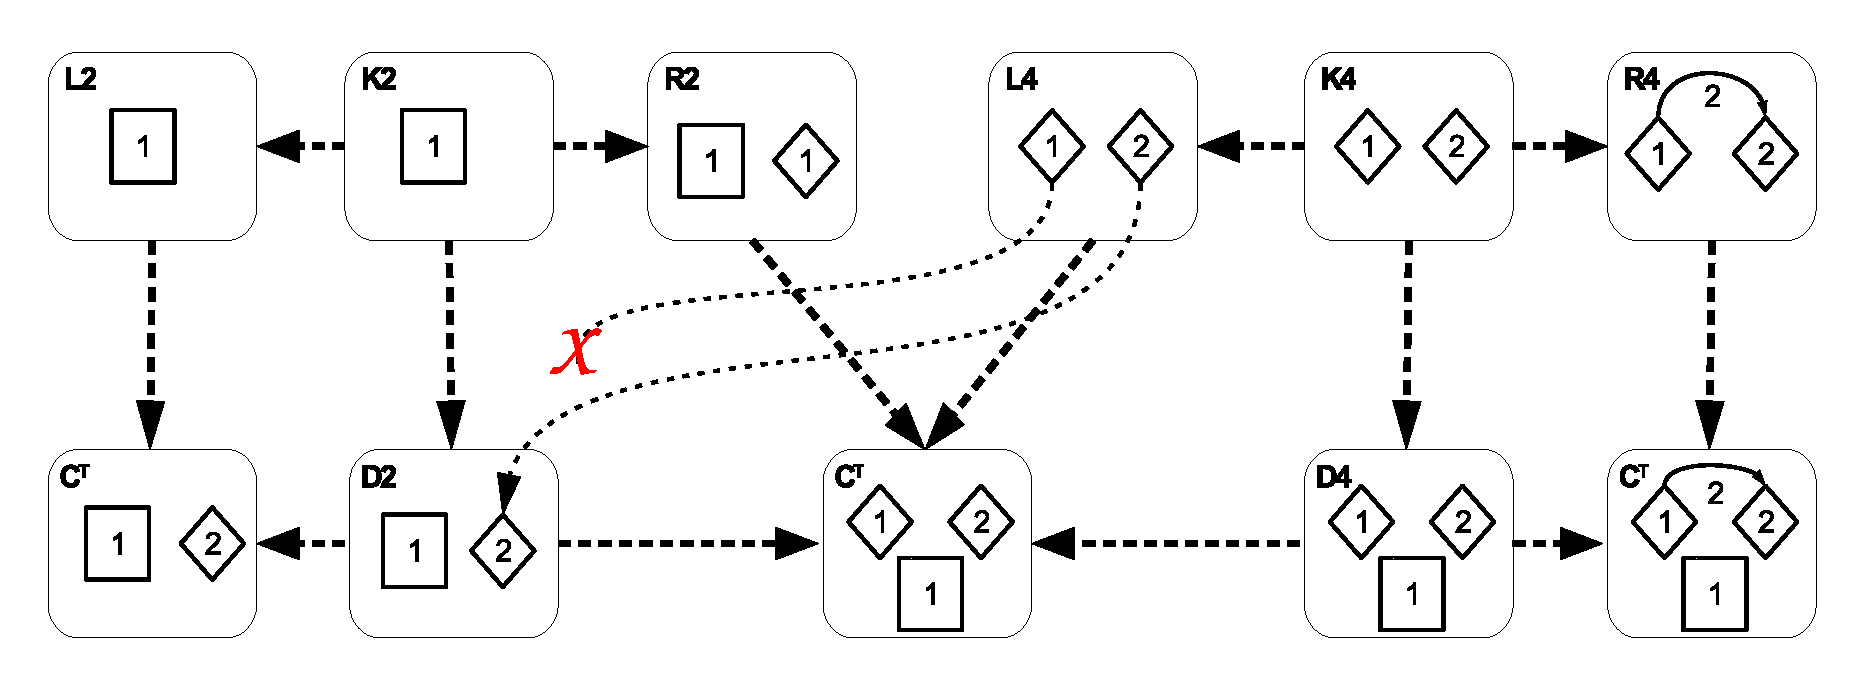
\includegraphics[scale=0.48]{images/process/unconditional-relation/dependency}}
  \caption{Unconditional causal dependency situation}\label{fig:process:unconditional-relation:dependency}
\end{figure}
\end{example}

Regarding both unconditional and conditional weak conflict relations, their definitions are based on the following intuition:

  \begin{intuition} An action $a_1$ is in \emph{weak} conflict with an action $a_2$ if either $a_1$ deletes something that is needed by $a_2$ to be applied (unconditional weak conflict) or creates something that is both forbidden by a NAC of $a_2$ and not deleted before the application of $a_2$ (conditional weak conflict). In both cases, we have that $a_2$ can not be applied once $a_1$ has been applied, in other words, $a_2$ can only be applied before $a_1$.
\end{intuition}

\begin{definition}[Unconditional Weak Conflict Relation\footnote{Also called Delete-Use Relation.}]\label{def:unconditional-conflict} Given \doublyTypedGraphGrammarCore{} a strongly safe graph grammar. Let $a_1, a_2 \in P$, $a_1 \ne a_2$, \mbox{$e_1, e_2 \in $ \coreGraph{}} and $e_1 \ne e_2$. Then: 

  \begin{enumerate}
    \item The action $a_1$ is in \emph{direct weak conflict} with $a_2$, written $a_2 <_{du} a_1$, iff \mbox{$\not\exists h_{21} : L_2 \rightarrow D_1$} s.t. \mbox{$d_1 \circ h_{21} = pre_2$}.

      \diagram{
          & & N_1 & & N_2 & & \\
        R_1 & K_1\ar[l]\ar[r]\ar[d] & L_1\ar[u]\ar[dr]_{pre_1} & & L_2\ar[u]\ar[dl]^{pre_2}\ar@{.>}@/_1.1pc/[dlll]|{|}_<<<<{h^{21}} & K_2\ar[l]\ar[r]\ar[d] & R_2\\
       & D_1\ar[rr]_{d_1} & & C^T_{|L_1L_2} & & D_2\ar[ll] &}
   \item The \emph{weak conflict relation between actions} $\leq_{du}$ of $P$ is the reflexive and transitive closure of the direct weak conflict.
   \item The element $e_2$ is \emph{in direct weak conflict} with $e_1$, written $e_2 <_{du} e_1$, iff there are actions $a_1$ and $a_2$ that respectively create $e_1$ and $e_2$ and $a_2 \leq_{du} a_1$.
   \item The \emph{weak conflict relation between elements} $\leq_{du}$ of $N(C^T) \cup E(C^T)$ is the reflexive and transitive closure of the direct weak conflict.
   \item The \emph{weak conflict relation} of a strongly safe grammar is defined by transitive and reflexive closure of the unions of relations $\leq_{du}$ for $P$ and $N(C^T) \cup E(C^T)$.

  \end{enumerate}
\end{definition}

\begin{example}[Unconditional Weak Conflict Example] Figure~\ref{fig:process:unconditional-relation:conflict} shows a delete-use between the actions $a_1$ and $a_2$ of the strongly safe grammar depicted in Figure~\ref{fig:process:unconditional-relation}.

  Again, both actions have valid graph transformations, now for the overlapping of $pre_1$ and $pre_2$ on $C^T$, but it is not possible to find a morphism from $L_2$ to $D_1$ satisfying the conditions on Definition~\ref{def:unconditional-conflict}.
\begin{figure}[!ht]
  \centering
  \fbox{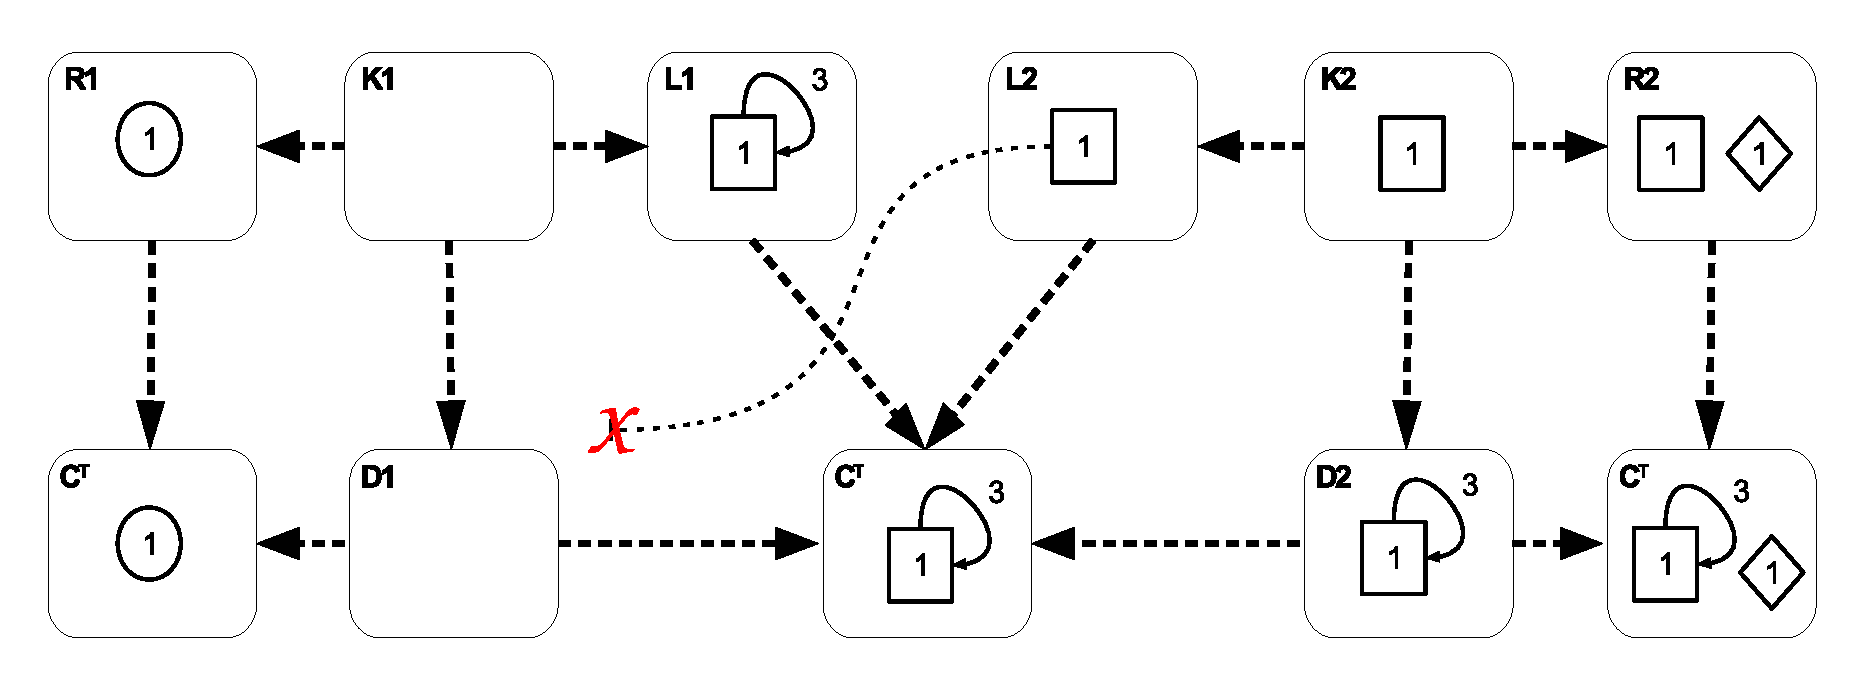
\includegraphics[scale=0.48]{images/process/unconditional-relation/conflict}}
  \caption{Unconditional weak conflict situation}\label{fig:process:unconditional-relation:conflict}
\end{figure}
\end{example}

\begin{definition}[Unconditional Occurrence Relation] Given \doublyTypedGraphGrammarCore{} a strongly safe graph grammar, let $\leq_{pu}$ and $\leq_{du}$ be the unconditional dependency and unconditional weak conflict relations of this grammar for $P \cup N(C^T) \cup E(C^T)$. Then the \emph{unconditional occurrence relation} of GG is the reflexive and transitive closure of \mbox{$\leq_{pu} \cup \leq_{du}$}.
\end{definition}

Similarly to the existential relation,~\cite{Ribeiro1996} proved that if this relation is a partial order, then it is possible to apply all actions of its underlying grammar in any total order that respects the partial order. Again, this condition is not sufficient if the rules may be equipped with NACs, as it was also shown to be equivalent to the existential relation.

\fi

\important{review the rest of this section after the removal of leila's relations}

\begin{example}[Unconditional Relations] \tinytodo{Create at least one more rule to show the transitive closure working?} For the strongly safe grammar depicted on Figure~\ref{fig:process:unconditional-relation} we have the following relations: 

\begin{itemize}
  \item produce-use dependencies: $a_1 <_{pu} a_3$, $a_2 <_{pu} a_3$, $a_2 <_{pu} a_4$. Therefore, the unconditional dependency relation for the actions is $a_1 \leq_{pu} a_3$, $a_2 \leq_{pu} a_3$, $a_2 \leq_{pu} a_4$. 
  \item delete-use conflicts: $a_2 <_{du} a_1$. Therefore, the unconditional weak conflict relation for the actions is $a_2 \leq_{du} a_1$.
  \item unconditional occurrence relation: $a_1 \leq a_3$, $a_2 \leq a_3$, $a_2 \leq a_4, a_2 \leq a_1$.
\end{itemize}

\begin{figure}[!ht]
  \centering
  \begin{subfigure}[t]{.5\textwidth}
    \centerline{\fbox{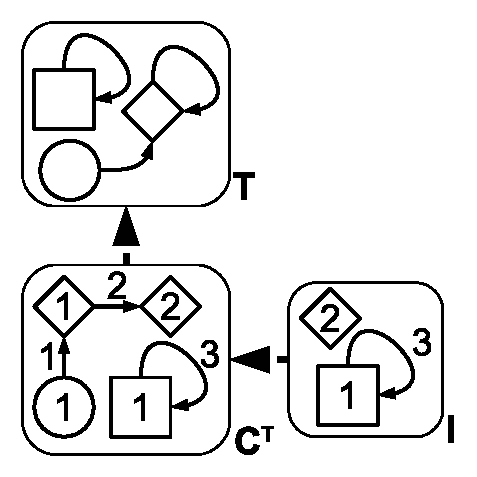
\includegraphics[scale=0.5]{images/process/unconditional-relation/core-graph}}}
    \caption{Core and initial graphs}\label{fig:process:unconditional-relation:core-graph}
  \end{subfigure}

  \begin{subfigure}[t]{.2\textwidth}
    \centerline{\fbox{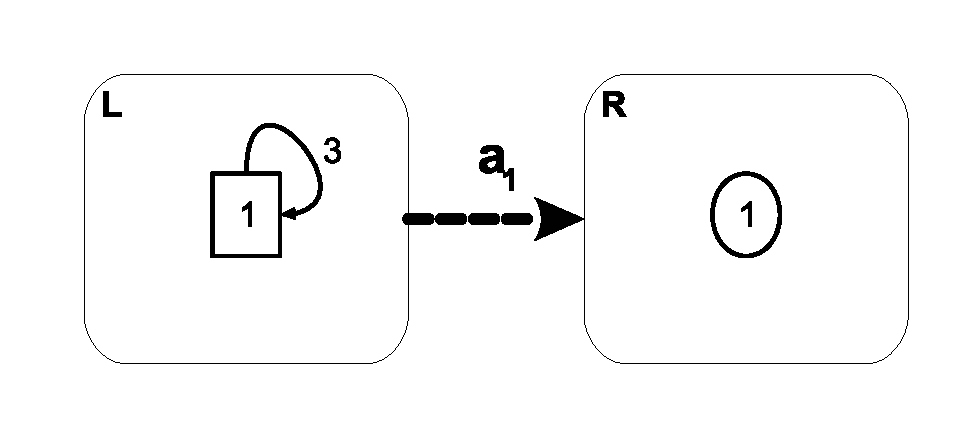
\includegraphics[scale=0.5]{images/process/unconditional-relation/a1}}}
    \caption{Action $a_1$}\label{fig:process:unconditional-relation:a1}
  \end{subfigure}%
  \begin{subfigure}[t]{.2\textwidth}
    \centerline{\fbox{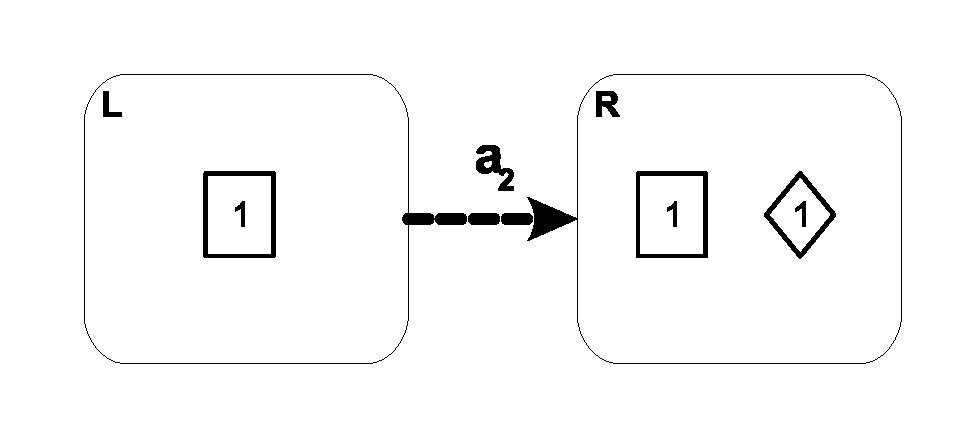
\includegraphics[scale=0.5]{images/process/unconditional-relation/a2}}}
    \caption{Action $a_2$}\label{fig:process:unconditional-relation:a2}
  \end{subfigure}%
  \begin{subfigure}[t]{.3\textwidth}
    \centerline{\fbox{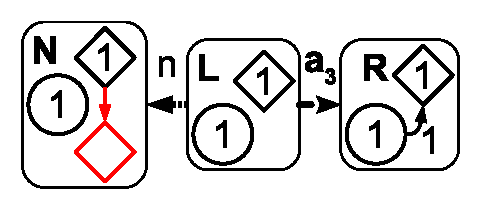
\includegraphics[scale=0.5]{images/process/unconditional-relation/a3}}}
    \caption{Action $a_3$}\label{fig:process:unconditional-relation:a3}
  \end{subfigure}%
  \begin{subfigure}[t]{.2\textwidth}
    \centerline{\fbox{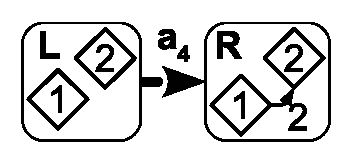
\includegraphics[scale=0.5]{images/process/unconditional-relation/a4}}}
    \caption{Action $a_4$}\label{fig:process:unconditional-relation:a4}
  \end{subfigure}
  \stepcounter{doubly-typed-grammar-counter}
  \caption{Strongly safe grammar GG\arabic{doubly-typed-grammar-counter}}\label{fig:process:unconditional-relation}
\end{figure}

  In order to know if all the actions of a strongly safe grammar without NACs can be applied, it would be sufficient to check whether the unconditional occurrence relation is a partial order.

  In particular, if we do not consider the NACs for the grammar in Figure~\ref{fig:process:unconditional-relation}, any total order of action compatible with the partial order given by the unconditional occurrence relation would be a valid sequentialization of this grammar. As an example, $[a_2, a_1, a_3, a_4]$ and $[a_2, a_4, a_1, a_3]$ are valid serializations (without NACS) for this grammar. 
  
  However, not all previous serializations are valid when NACs come into play. Specifically, the sequence $[a_2, a_4, a_1, a_3]$ is not valid, because if $a_4$ is applied before $a_3$ it creates $\curvearrowleft_2$, triggering the NAC of $a_3$ which can no longer be applied.

\end{example}

\begin{remark}[Existential and Unconditional Occurrence Relations] Since the \emph{existential} and \emph{unconditional occurrence relations} where shown to be equivalent by~\cite{Ribeiro1996}, we will only one of them, the \emph{existential relation}, as the standard relation without without NACs from now on, as it was originally defined for DPO grammars.

  However, we were heavily inspired by the structure of the \emph{unconditional causal dependency} and \emph{unconditional weak conflict relations} to define the relations with NACs.
\end{remark}

\section{Relations within Strongly Safe Graph Grammars with NACs}

The existential relation presented in the previous section is always concrete. This means that if an action is dependent on (conflicting with) another one, it happens because the one of them creates (resp. deletes) at least one of the concrete elements necessary for the other to be applied (resp. prevented of being applied).

Moreover, the existential relation must always be respected whenever we try to find a total order in which all the actions of a strongly safe grammar are applicable. However, for grammars equipped with NACs it is necessary to include the conflicts and dependencies created by NACs in this relation.

The problem here is that we can not just add the conflicts and dependencies caused by NACs directly into the existential relation \important{(as was the case for their unconditional counterparts in the unconditional occurrence relation)} because they are potential. In other words: according to the total order of application chosen among the existential relation possibilities, a conflict (dependency) may or may not happen.

In fact, according to the possible application orders, such dependencies and conflicts may be characterized as \emph{concrete}, they will happen no matter the chosen order; \emph{non existent}, they will never happen no matter the order; or \emph{abstract}, they may occur in only in some total orders. \important{maybe extract this to a definition and also add the explanation for potential}

\begin{example}[Interaction between existential relation and NACs]
Let $a_1, a_2, a_3$ be three actions of the same strongly safe grammar. Suppose that $a_1$ creates elements used by $a_2$ and $a_2$ creates elements used by $a_3$, therefore by the existential relation we know that $a_1 \leq_e a_2 \leq_e a_3$. Now suppose that when $a_2$ is applied, it creates an element that would be forbidden by a NAC of $a_1$ and also that $a_3$ deletes this element. Following the classical notions of dependency and conflict with NACs, as shown in
  definitions~\ref{def:classic-dependency} and~\ref{def:classic-conflict}, $a_2$ would cause a (potential) produce-forbid conflict on $a_1$ $(a_1 <_{pf} a_2)$, while $a_1$ would be (potentially) dependent by delete-forbid on $a_3$ $(a_3 <_{df} a_1)$. By adding these produce-forbid and delete-forbid directly to the existential relation we would have the situation depicted in Figure~\ref{fig:process:order:occurrence-relation-fail}. It is easy to see that the resulting relation is not a partial order, therefore there can be no total ordering for this set of actions.
\begin{figure}[!ht]
  \centering
  \fbox{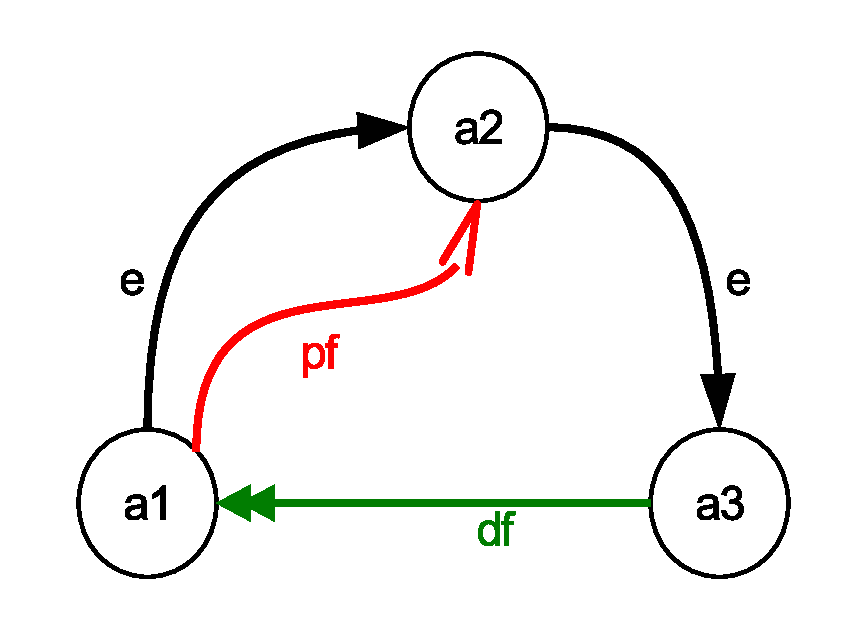
\includegraphics[scale=1]{images/process/order/occurrence-relation-fail}}
  \caption{Graph of relations}\label{fig:process:order:occurrence-relation-fail}
\end{figure}

However, looking at the existential relation, we can affirm that this configuration ensures that neither the conflict nor the dependency exist in any concrete execution of this grammar. For the conflict, this happens because $a_2$ can only happen after $a_1$, thus the element forbidden by the NAC of $a_1$ can only exist after $a_1$ itself was already applied. Likewise, the dependency that is identified because $a_3$ deletes the element that would be forbidden by the NAC of $a_1$ does not exist either.\tinytodo{Draw examples for non existent (last paragraph), concrete and potential dependencies/conflicts?}
\end{example}

We already know that at least the existential relation must be a partial order in order to be possible to apply all the actions of a grammar. Nevertheless, the following problem remains to be solved:

\begin{intuition}
  Given a strongly safe grammar \doublyTypedGraphGrammarCore{} with at least two actions $a_1, a_2 \in P$ in a potential delete-forbid or a potential produce-forbid situation, under which circumstances this dependency or conflict exists and must be considered in the ordering of actions application?
\end{intuition}

In the following, we categorize this conflicts and dependencies according to their triggering elements and their pertinence into the existential relation in order to solve this problem.

\begin{definition}[Delete-Forbid Relation in Strongly Safe Graph Grammars]\label{def:delete-forbid-strong} Let \doublyTypedGraphGrammarCore{} be a strongly-safe graph grammar, where $P$ is a set of actions with incremental, non-trivially triggered NACs only.

\diagram{
  \mathbf{a_1} & & N^{-1}_1 & & N_2\ar@{.>}@/_1.1pc/[ddllll]_<<<<{q} & & \mathbf{a_2}\\
  L_1\ar[d] & K_1\ar[d]\ar[l]\ar[r] & R_1\ar[u]^{n_1}\ar[dr]_{post_1} & & L_2\ar[u]_{n_2}\ar@{.>}@/_1.1pc/[dlll]_<<<<{h_{21}}\ar[dl]^{pre_2} & K_2\ar[l]\ar[r]\ar[d] & R_2\\
     C^T_{|L_1D_1} & D_1\ar[rr]_{d_1}\ar[l]^{e_1} & & C^T_{|R_1L_2} & & D_2\ar[ll] &}
\hfill

  Let $a_1, a_2 \in P$ be in a potential delete-forbid dependency according to the diagram above, where $a_1$ deletes from graph $C^T_{|L_1D_1}$ an element $x \in N($\coreGraph$) \cup E($\coreGraph$)$ which is the triggering element of a NAC $N_2$ of $a_2$ for the extended match $e_1 \circ h_{21}$. This delete-forbid dependency is:

\begin{itemize}
  \item \emph{concrete}: iff $(x \leq_e a_2) \lor (x \in I^{C^T})$;
  \item \emph{abstract}: iff $(\exists a_3 \in P \mid x \in R_3 - K_3)$ $\land$ $(x \not\leq_e a_2)$ $\land$ $(a_2 \not\leq_e x)$;%\tinytodo{ $(x,a_2)$ or $(a_3, a_2)$?}
  \item \emph{non existent}: otherwise.
\end{itemize}

  Two elements $x, y \in N(C^T) \cup E(C^T)$ are in a delete-forbid dependency if there are actions $a_1,a_2$ such that (1) $a_1 <_{df} a_2$ and (2) $a_1$ creates $x$ and $a_2$ creates $y$. In this case use say that $x <_{df} y$.

  The delete-forbid between two elements has the same quality (concrete, abstract, non existent) as the one between the actions involved in this dependency.
\end{definition}

\important{explain concrete / abstract / non-existent}

The delete-forbid dependency found in the diagram can have different classifications according to the existential relation of its underlying strongly safe graph grammar and also to the existence (or not) of the triggering element in the initial graph. Thus, we need to demonstrate that

\important{Rethink:}

\begin{thm} The definition~\ref{def:delete-forbid-strong} captures all cases of a \emph{delete-forbid} in strongly safe graph grammars.
\end{thm}

\begin{proof} Given actions $a_1,a_2 \in P$ in \emph{delete-forbid} and the element $x \in C^T$ which is the triggering element of this dependency, we may have that:
\hfill
\begin{description}[style=nextline,leftmargin=*]

  \item [Triggering element is present on the initial graph:]
Let $x$ be not created by any action in $P$, meaning that $x$ is present on the initial graph: $x \in I^{C^T}$. In such configuration, the delete-forbid is \emph{concrete}, given that $x$ exists before the application of $a_2$ (or any other action), preventing the application of the action until it gets deleted. Therefore, we have $a_1 <_{df} a_2$.

  \item [Triggering element is related to the action:] If $a_2 \leq_e x$, it means that $x$ was either created by $a_2$ or by another action that must to occur after $a_2$. In this configuration the delete-forbid dependency is \emph{non existent} as the element $x$ can not exist to trigger $N_2$ before $a_2$ was already applied.

    On the other hand, if $x \leq_e a_2$, it means that $x$ must exist at some moment before $a_2$ is applied. In this configuration, we have that $x$ must be deleted in order for $a_2$ to be applied. Since $a_1$ is the only action that deletes $x$ (otherwise the underlying grammar would not be a strongly safe grammar) this delete-forbid is \emph{concrete} and we have that $a_1 <_{df} a_2$.

\item [Triggering element is not related to the action:]
  Let $x$ be not related to $a_2$, but created by a third action $a_3 \in P$ (notice that in this configuration we have that $a_3 <_{e} a_1$).

    Let $a_3$ be not related to $a_2$, in which case we have that $a_1$ and $a_2$ \emph{would be} in a concrete delete-forbid dependency if $a_3$ was applied before $a_2$. On the other hand, the same dependency \emph{would be} non existent if $a_3$ was applied after $a_2$. We name this situation an \emph{abstract} produce-forbid dependency and represent it by $[a_1 <_{df} a_2$ | $a_2 < a_3]$ or $a_2 \not\in [a_3 \ldots a_1]$.

%    in which case we have an \emph{abstract} delete-forbid $a_1 <_{df} a_2$ conditioned to $a_3$: in a configuration where $a_3$ is applied before $a_2$ the produce-forbid exists, otherwise it does not. We will represent this \emph{abstract delete-forbid dependency} as .

Now, let $a_3$ be related to $a_2$. In this configuration, we have that $a_2$ would be related to $x$, as $a_3$ creates $x$, which corresponds to our second case.
\end{description}
\end{proof}

\begin{definition}[Produce-Forbid in Strongly Safe Graph Grammars]\label{def:produce-forbid-strong} Given \doublyTypedGraphGrammarCore{} a strongly safe graph grammar, where $P$ is a set of actions with incremental, non-trivially triggered NACs only.

\diagram{
  \mathbf{a_1^{-1}}& & N_1 & & N_2\ar@{.>}@/_1.1pc/[ddllll]_<<<<{q} & & \mathbf{a_2}\\
  R_1\ar[d] & K_1\ar[d]\ar[l]\ar[r] & L_1\ar[u]^{n_1}\ar[dr]_{pre_1} & & L_2\ar[u]_{n_2}\ar@{.>}@/_1.1pc/[dlll]_<<<<{h_{21}}\ar[dl]^{pre_2} & K_2\ar[l]\ar[r]\ar[d] & R_2\\
     C^T_{|R_1D_1} & D_1\ar[rr]_{e_1}\ar[l]^{d_1} & & C^T_{|L_1L_2} & & D_2\ar[ll] &}
\hfill

  Let $a_1,a_2 \in P$, be in a produce-forbid conflict according to the diagram above, where on $a_1$ creates on $C^T_{|R_1D_1}$ an element $x \in N(C^T) \cup E(C^T)$ which is the triggering element of a NAC $N_2$ of $a_2$ for the extended match $d_1 \circ h_{21}$. This produce-forbid conflict is:

\begin{itemize}
  \item \emph{concrete}: iff $(\not\exists a_3 \in P \mid x \in L_3 - K_3) \land (x \leq_e a_2 \lor a_2 \not\leq_e x)$; %iff $(x \leq_e a_2) \land (\not\exists a_3 \mid x \in L_3 - K_3)$ or $(x,a_2),(a_2,x) \not\in \leq_ei \land (\not\exists a_3 \mid x \in L_3 - K_3)$\tinytodo{summarize this: $\not\exists a_3 \mid x \in L_3 - K_3 \land a_2\not\leq_e x$?}
  \item \emph{abstract}: iff $(\exists a_3 \in P \mid x \in L_3 - K_3) \land (a_3 \not\leq_e a_2) \land (a_2 \not\leq_e a_3)$;
  \item \emph{non existent}: otherwise.
\end{itemize}

  Two elements $x, y \in N(C^T) \cup E(C^T)$ are in a produce-forbid conflict if there are actions $a_1,a_2$ such that (1) $a_2 <_{pf} a_1$ and (2) $a_1$ creates $x$ and $a_2$ creates $y$. In this case use say that $y <_{pf} x$.

  The produce-forbid between two elements has the same quality (concrete, abstract, non existent) as the one between the actions involved in this conflict.
\end{definition}

  Similarly to the dependency situation, the produce-forbid conflict can have different meanings according to the existential relation of its grammar. Nonetheless, once we are dealing with strongly safe grammars and this element is created by one of the actions involved in the conflict, we do not have to worry about the initial graph. Thus, we need to demonstrate that:

\begin{thm} The definition~\ref{def:produce-forbid-strong} captures all cases of a \emph{produce-forbid} in strongly safe graph grammars.
\end{thm}

\begin{proof} Given actions $a_1,a_2 \in P$ in \emph{produce-forbid} and the element $x \in C^T$ which is the triggering element of this conflict, we may have that:
\hfill

\begin{description}[style=nextline,leftmargin=*]
  \item[Triggering element is related to the action:]
    Let $a_2 \leq_e x$, which means that $x$ was created by $a_2$ or by another action that must occur after $a_2$ has been applied. In such a configuration, the produce-forbid conflict is \mbox{non existent} as the element $x$ can not exist to trigger $N_2$ before the application of $a_2$.

    Now let $x \leq_e a_2$, which means that $x$ existed before $a_2$ was applied, which leads to two possible sub cases:

    \begin{itemize}
      \item Assume that there is no other action $a_3$ which deletes $x$. In this situation, we have both that the triggering element $x$ exists before the application of $a_2$ and that $x$ is never deleted. Therefore, the produce-forbid between $a_1$ and $a_2$ is \emph{concrete} and we have that the $a_2 <_{pf} a_1$.
      \item Assume that there exists a third action $a_3 \in P$ which deletes $x$. This means that, even though $a_1$ and $a_2$ are in a concrete produce-forbid conflict, this conflict can be ``annulated'' by the application of $a_3$, which must then happen before $a_2$. Notice that in this configuration we will probably have that $a_3 <_{df} a_2$\tinytodo{review this, the ``dependency'' may not occur but the order of application must contain $a_3 < a_2$}.
    \end{itemize}

  \item[Triggering element is not related to the action:]
    Let $a_2$ be not related to $x$ in the existential relation.

    Suppose that there is no other action $a_3$ which deletes $x$, then we know for a fact that once $a_1$ has been applied and $x$ has been created it will no longer be possible to apply $a_2$. Therefore, this produce-forbid is \emph{concrete} and we have that $a_2 <_{pf} a_1$.

    On the other hand, suppose that there is an action $a_3$ which deletes $x$ and $a_3$ not related to $a_2$ by the existential, thus we have $a_1 <_e a_3$. In this configuration, we have an \emph{abstract} conflict, in the sense that $a_2$ can not be applied after $a_1$ has been applied, unless $a_3$ is also applied before $a_2$, disabling the produce-forbid conflict. We represent this \emph{abstract} produce-forbid conflict as \mbox{$[a_2 <_{pf} a_1$ | $a_3 < a_2]$} or \mbox{$a_2 \not\in [a_1\ldots a_3]$}.
\end{description}
\end{proof}

\begin{example}[Conditional Relations] Consider the strongly safe grammar show in Figure~\ref{fig:process:order} (the core, typed and initial graphs were omitted). 
  
\begin{figure}[!ht]
  \centering
  \begin{subfigure}[t]{.2\textwidth}
    \centerline{\fbox{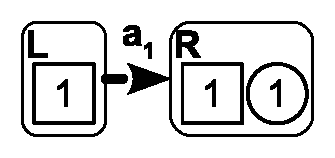
\includegraphics[scale=0.6]{images/process/order/a1}}}
    \caption{Action $a_1$}\label{fig:process:order:a1}
  \end{subfigure}%
  \begin{subfigure}[t]{.2\textwidth}
    \centerline{\fbox{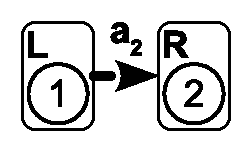
\includegraphics[scale=0.6]{images/process/order/a2}}}
    \caption{Action $a_2$}\label{fig:process:order:a2}
  \end{subfigure}%
  \begin{subfigure}[t]{.3\textwidth}
    \centerline{\fbox{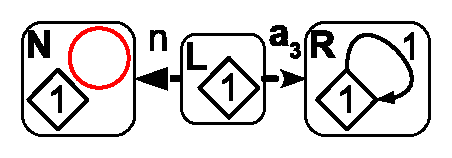
\includegraphics[scale=0.6]{images/process/order/a3}}}
    \caption{Action $a_3$}\label{fig:process:order:a3}
  \end{subfigure}%
  \begin{subfigure}[t]{.2\textwidth}
    \centerline{\fbox{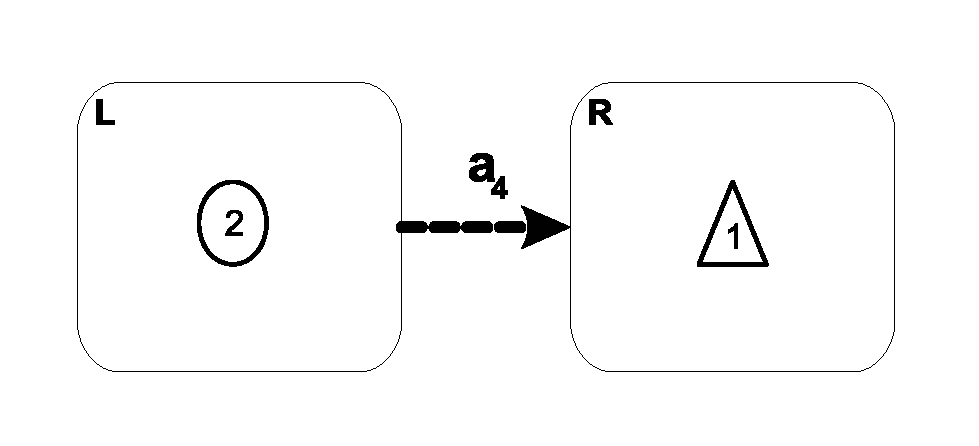
\includegraphics[scale=0.6]{images/process/order/a4}}}
    \caption{Action $a_4$}\label{fig:process:order:a4}
  \end{subfigure}
  \stepcounter{doubly-typed-grammar-counter}
  \caption{Strongly safe grammar GG\arabic{doubly-typed-grammar-counter}}\label{fig:process:order}
\end{figure}

  The existential relation of this grammar is: $a_1 \leq_e a_2, a_2 \leq_e a_4, a_1 \leq_e a_4, a_3 \leq_e a_3$. Without the NACs, any sequentialization where the order $a_1 < a_2 < a_4$ is maintained would be valid, such as $[a_1, a_2, a_3, a_4]$, $[a_1,a_3,a_2,a_4]$, $[a_3, a_1, a_2, a_4]$ and $[a_1,a_2,a_4,a_3]$.

  However, as this grammar have NACs, the following conditional conflicts and dependencies have been identified:
\begin{itemize}
  \item delete-forbids: $a_4 <_{df} a_3$ caused by the deletion of $\Circle_2$.
  \item produce-forbids: $a_3 <_{pf} a_1$ caused by creation of $\Circle_1$, and $a_3 <_{pf} a_2$ caused by the creation of $\Circle_2$.
\end{itemize}

  Notice that, despite of the fact that $a_2$ deletes $\Circle_1$, which triggers the NAC of $a_3$, $a_2 <_{df} a_3$ is not a delete-forbid dependency because $a_2$ also creates $\Circle_2$, an element that still triggers the same NAC. Therefore the transformations when searching for the dependency between $a_2$ to $a_3$ are not valid.

  None of these conflicts or dependencies is \emph{concrete}, depending on how the orders are applied according to the existential relation and unconditional occurrence relation to exist.
  
  This situation is summarized in Figure~\ref{fig:process:order:cycle}, where the existential relation, the conflicts and dependencies are represented (without the explicit representation of transitivity and reflexivity). At first, if we are consider all the relations \textbf{as they are calculated}, there is no possible sequentialization for this actions, denoted by the cycle in the ordering graph.

\begin{figure}[!ht]
  \centering
  \fbox{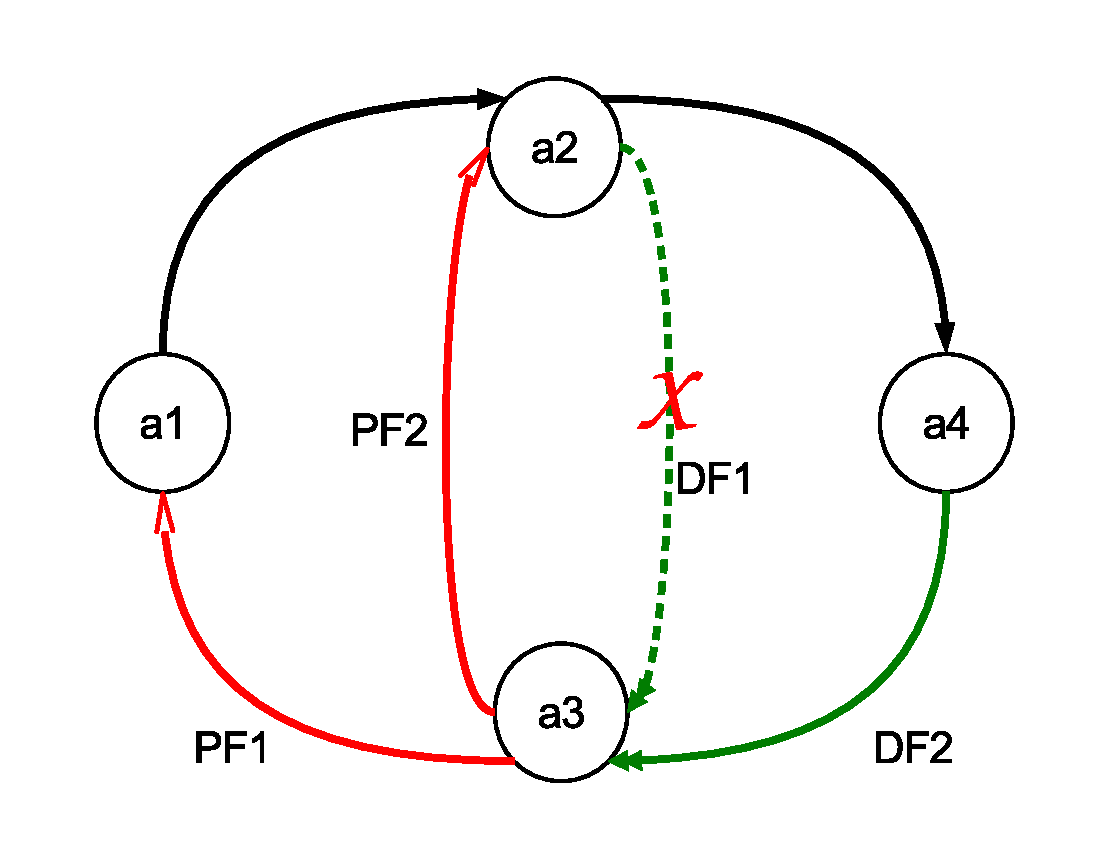
\includegraphics[scale=1]{images/process/order/cycle}}
  \caption{Cycle due to conditional conflicts and dependencies}\label{fig:process:order:cycle}
\end{figure}

  Regarding the element $\Circle_1$, we have an abstract produce-forbid conflict as $a_3$ can be applied before $a_1$ creates it or after $a_2$ deletes it. Thus it is possible to apply $a_3$ as long as $a_3 \not\in [a_1\ldots a_2]$. %\mbox{$[a_3 <_{pf} a_1$ $|$ $a_2 < a_3]$}.

  As for the element $\Circle_2$, we have an abstract produce-forbid conflict \mbox{$[a_3 <_{pf} a_2$ $|$ $a_4 < a_3]$} and an abstract delete-forbid dependency \mbox{$[a_3 < a_2$ $|$ $a_4 <_{df} a_3]$}. Since the produce-forbid and the delete-forbid act on the same element, we can simply say that \mbox{$[a_3 <_{pf} a_2$ $|$ $a_4 <_{df} a_3]$}. In this configuration, $a_3$ can be applied as long as $a_3 \not\in [a_2\ldots a_4]$.

  In fact, we have that this particular grammar can be executed in any total ordering of its existential relation $a_1 \leq_e a_2, a_2 \leq_e a_4, a_1 \leq_e a_4, a_3 \leq_e a_3$ that also respects the \emph{restrictions} $a_3 \not\in [a_1\ldots a_2]$ and $a_3 \not\in [a_2\ldots a_4]$.

  There exist two such sequentializations of this existential relation: $[a_3, a_1, a_2, a_4]$ and $[a_1,a_2,a_4,a_3]$.
\end{example}

\begin{remark}[Abstract Dependencies and Conflicts] The existence of an abstract produce-forbid conflict caused by an element $x$ is conditioned to the existence of an action which deletes $x$.

  Given an action $a_1$ which creates $x$, an action $a_2$ whose NAC forbids $x$ and provided a configuration where $a_1$ was applied before $a_2$, we have that $a_2$ can be applied only after an action $a_3$ which deletes $x$ has been applied.

  However, $a_3$ may also cause a new produce-forbid conflict on $a_2$ by creating a new element $y$ which is also forbidden by a NAC of $a_2$, on which case $a_2$ can only be applied of there is another action $a_4$ which ``turns off'' the conflict caused by $a_3$.

  In general, for each abstract produce-forbid conflict $a_2 <_{pf} a_1$ caused by an element $x$, we have that $a_2$ must be successfully applied before $a_1$ or after an action $a_{j}$ where $a_i$ deletes $x$ and $a_i \leq a_j$.

  Analogously, for each abstract delete-forbid conflict $a_1 <_{df} a_2$ caused by an element $x$, we have that $a_2$ must be successfully applied after $a_1$ or before an action $a_j$ where $a_i$ creates $x$ and $a_j \leq a_i$.
\end{remark}

\begin{definition}[Occurence Relation] Given a strongly safe grammar \doublyTypedGraphGrammarCore{}, let $[\leq_{df}]$ be the set of all its \emph{concrete} delete-forbids and $[\leq_{pf}]$ be the set of all its \emph{concrete} produce-forbids. Then, its occurrence relation $\leq_o$ of $(P \cup N(C^T) \cup E(C^T))$ is defined as the transitive and reflexive closure of \mbox{$\leq_{e}$ $\cup$ $[\leq_{df}]$ $\cup$ $[\leq_{pf}]$}.
\end{definition}

\begin{definition}[Occurence Relation Restrictions] Given a strongly safe grammar \doublyTypedGraphGrammarCore{}, its \emph{occurrence relation restrictions} is the set $R$ containing all its abstract produce-forbid conflicts and delete-forbid dependencies.
\end{definition}

\begin{definition}[Occurrence Graph Grammars] Let \doublyTypedGraphGrammarCore{} be a strongly safe graph grammar. $GG$ is an \emph{occurrence graph grammar} iff:

  \important{add corradini's original definition and extend it. Do not forget to add initial and final graphs}
  \begin{enumerate}
    %\item acyclic existential relation: $\forall a \in P$: $\leq_e$ is antisymmetric;
    \item acyclic occurrence relation: $\forall a \in P$: $\leq_o$ is antisymmetric;
    \item there is at least one serialization of the actions $a_1,\ldots,a_n \in P$ that respects the occurrence relation restrictions.
  \end{enumerate}
\end{definition}

As was said in the beginning of this chapter, the idea is that an occurrence graph grammar is a suitable to describe the semantics of a graph grammar, in the sense that it represents both all possible states and changes of states that is also a graph grammar.

The first condition of the definition assures that it is possible to find a sequence of actions that respects both the order of creation and deletion of elements given by the existential relation and the order imposed by the concrete produce-forbids and delete-forbids of the grammar. In other words, it assures that there is no cycle of conflicts and dependencies that can prevent the application of the grammar.

The second condition deals with the conflicts and dependencies induced by NACs that do not participate in the concrete relations and generate \emph{intervals} of actions in which specific inside of which specific actions can not be applied.
